% -*- Mode:TeX -*-


\documentclass[11pt,twoside,singlespace]{report}
%\pagestyle{plain}
%\pagestyle{headings}
%\lhead{\chaptermark}

\usepackage{amssymb,amsmath} % better maths commands
\usepackage{graphicx}
\usepackage{verbatim}  % allows 'comment' environment, which is useful for commenting out multi-line sections
%\usepackage{txfontsb}
\usepackage{mymanual}
\graphicspath{{graphics/}}
\usepackage[usenames]{color}
%\maxtocdepth{section}
\usepackage[sort&compress,numbers]{natbib} % better citations
\usepackage{fancyhdr}
%\usepackage[nottoc,notlot,notlof]{tocbibind}
\usepackage{url}
\usepackage{hyperref}
\hypersetup{colorlinks=true,linkcolor=blue}

\newcommand{\vv}{\upsilon}
\newcommand{\vect}[1]{{\mathbf #1}}
\newcommand{\sfincs}{{\ttfamily sfincs}}
\newcommand{\sfincsScan}{{\ttfamily sfincsScan}}
\newcommand{\sfincsPlot}{{\ttfamily sfincsPlot}}
\newcommand{\sfincsScanPlot}{{\ttfamily sfincsScanPlot}}
\newcommand{\PETSc}{{\ttfamily PETSc}}
\newcommand{\HDF}{{\ttfamily HDF5}}
\newcommand{\netCDF}{{\ttfamily netCDF}}
\newcommand{\superludist}{{\ttfamily superlu\_dist}}
\newcommand{\mumps}{{\ttfamily mumps}}
\newcommand{\python}{{\ttfamily python}}
\newcommand{\parlink}[1]{{\ttfamily \hyperlink{#1}{#1}}}
\newcommand{\Ntheta}{\parlink{Ntheta}}
\newcommand{\Nzeta}{\parlink{Nzeta}}
\newcommand{\Nxi}{\parlink{Nxi}}
\newcommand{\Nx}{\parlink{Nx}}
\newcommand{\NL}{\parlink{NL}}
\newcommand{\vmec}{{\ttfamily vmec}}
\newcommand{\dkes}{{\ttfamily dkes}}
\newcommand{\todo}[1]{\textcolor{red}{To do: #1}}

\graphicspath{{figures/}}

% uncomment the following line to remove all graphics (for faster compiling)
%\renewcommand{\includegraphics}[2][x]{}

\newcommand{\boldkappa}{{\mathbf \kappa}}

\setlength{\oddsidemargin}{0.25in}	% 1.25in left margin
\setlength{\evensidemargin}{0.25in}	% 1.25in left margin (even pages)
\setlength{\topmargin}{0.0in}		% 1in top margin
\setlength{\textwidth}{6.0in}		% 6.0in text - 1.25in rt margin
\setlength{\textheight}{8.6in}		% Body ht for 1in margins

\setcounter{tocdepth}{1}
\begin{document}


\begin{center}

\vspace*{2in}

{\Huge SFINCS User Manual}

\vspace{4in}

{\Large Version 3}

\vspace{0.5in}

Revised May 21, 2015

\end{center}




%\pagestyle{plain}
\fancyhf{}
\cfoot{\thepage}
\tableofcontents

\clearpage


\pagestyle{fancy}
\fancyhf{}
\lhead[\thepage]{\leftmark}
\rhead[\leftmark]{\thepage}
%\lhead{\chaptermark}
\renewcommand{\chaptermark}[1]{\markboth{\sc{\chaptername\ \thechapter.\ #1}}{}}
\setlength{\headsep}{6pt}

\setlength{\parskip}{0pt plus 0pt minus 0pt}

% Main chapters go here:
\chapter{Overview}


The \sfincs~code is a freely available, open-source tool for solving neoclassical-type kinetic problems in nonaxisymmetric or axisymmetric plasmas
with nested toroidal flux surfaces.
As with other neoclassical codes, the input information used by \sfincs~is the equilibrium magnetic geometry together with the density, radial density gradient, temperature,
and radial temperature gradient of each species.  The code then solves a drift-kinetic equation for each species,
yielding the (gyro-angle averaged) distribution function.  Moments of the distribution function are computed such as the parallel
flow, bootstrap current, radial particle flux, radial heat flux, and variation of the density over a flux surface.  
These moments are all saved in the output file, and if you wish, you can also save the distribution function itself.
Optionally, a quasi-neutrality
equation can be solved at the same time as the drift-kinetic equations, yielding the self-consistent variation of the electrostatic potential on a flux surface.

The kinetic equations solved in \sfincs~have four independent variables: poloidal angle $\theta$, toroidal angle $\zeta$,
normalized speed $x = v / v_{thermal}$, and pitch angle $\xi = v_{||}/v$.  The third velocity coordinate (gyro-angle) does not appear
since gyro-averaged equations are solved.  The flux surface label (radius) coordinate is only a parameter, rather than a full independent variable,
since a radially local approximation is made.

This document discusses the practical use and operation of the code.  For more details about the specific equations implemented,
see the version 3 technical documentation available in the \path{sfincs/docs} directory.
Ref \cite{sfincsPaper} gives many details and some early physics results.

Often, the limiting factor for \sfincs~is the ability of the libraries \mumps~or \superludist~to factorize the preconditioner matrix, discussed in section \ref{sec:gmres}.
You may therefore find it useful to see the control parameters and error codes in the \mumps~user manual:
\url{http://mumps.enseeiht.fr/doc/userguide_5.0.0.pdf}.

This manual describes ``version 3'' of \sfincs.  
To preserve previous versions of the code that have been used for publications, two older versions of the
code called singleSpecies and multiSpecies are also present in the repository.  For both of these older versions,
both MATLAB and fortran editions exist which are independent of each other.  At present, version 3 exists
only in a fortran edition.

\section{Features}

\begin{itemize}

\item
Both self-species and inter-species collisions are treated using the most accurate linear operator available, the full linearized Fokker-Planck collision operator,
with no approximation of the field-particle term or expansion in mass ratio.  This collision operator conserves mass, momentum, and energy.

\item
Realistic experimental geometry can be simulated using an interface to \vmec.  Analytic model equilibria can also be used.

\item
Full coupling in the speed (or equivalently, kinetic energy) coordinate is retained, i.e. no monoenergetic approximation is made.  However,
if desired, \sfincs~can also be run in monoenergetic mode to compare with older codes.

\item
The code is formulated to permit solution of a wide variety of kinetic equations, whether or not phase space volume and/or energy are conserved, so individual terms can be turned on or off to examine their effect. 

\item
A variety of models for terms involving the radial electric field are available to allow comparison between models. 

\item
The code takes advantage of modern algorithms (GMRES) and parallelized libraries (\PETSc, \superludist, and \mumps).

\item
Efficient representation of velocity space is achieved using a pseudospectral method based upon non-classical orthogonal polynomials. \cite{speedGrids}

\item
Optional nonlinear terms in the kinetic equation (involving both the non-Maxwellian distribution function and poloidal/toroidal electric field) can be included using Newton's method. 

\end{itemize}

\section{Limitations}

\begin{itemize}

\item
The \sfincs~code is radially local, in the sense that it approximates 
the radial derivative of the distribution function $\partial f/\partial \psi$ by
the derivative of a Maxwellian flux function $\partial f_M(\psi,x)/\partial \psi$.
This approximation is important for reducing the otherwise 5D space of independent variables $(\psi,\theta,\zeta,x,\xi)$
to a 4D space $(\theta,\zeta,x,\xi)$.
As a result, \sfincs~cannot compute certain finite-orbit-width effects that occur when the radial extent of the particle orbits
between bounces or transits is not small compared to the scale of radial variation in the equilibrium.
Such finite orbit width effects are significant near the magnetic axis, and in strong transport barriers, such as the pedestal of a tokamak H-mode.

\item
Turbulence is neglected.  There are good theoretical reasons to expect that the neoclassical effects computed by \sfincs~should
decouple from turbulence, as detailed in \cite{AbelReview}.  However, this argument relies on an expansion in $\rho_* \ll 1$, and so may break down
in some circumstances when $\rho_*$ is not sufficiently small.

\item
It is assumed that nested toroidal magnetic surfaces exist. Thus, the code cannot accurately model regions of stochastic field,
magnetic islands, or open field lines.

\end{itemize}

\section{Geometry options}
In \sfincs, a variety of options are available for the magnetic field geometry.  The geometry can be read directly
from a {\ttfamily vmec wout}
file, or from the {\ttfamily .bc} format Boozer-coordinate data files used at the Max Planck Institute for Plasma Physics (IPP).
A general analytic model for the magnetic field is also available, given by equation (\ref{eq:Bmodel}),
as are several analytic models for LHD and W7-X in which 3 or 4 Fourier components are retained.
The primary switch for controlling the magnetic geometry in \sfincs~is the {\ttfamily geometryScheme} parameter
in the {\ttfamily geometryParameters} input namelist.
For more details about geometry options in \sfincs, see section \ref{sec:geometryParameters}.

\section{GMRES/KSP and preconditioning}
\label{sec:gmres}

At its heart, \sfincs~solves one or more large sparse linear systems $Ax=b$.  Here $b$ is a known right-hand side vector,
$A$ is a large (often millions $\times$ millions) known sparse matrix, and $x$ is the desired and unknown solution vector.
The direct way to solve such systems is to $LU$-factorize
the matrix $A$ into lower- and upper-triangular factors.
Once the $L$ and $U$ factors are found, the solution of the linear system
for any right-hand side vector can be rapidly obtained.  However, even if the original matrix is sparse, the $L$ and $U$ factors
are generally not sparse, and so a very large amount of memory can be required for a direct $LU$-factorization.

An alternative way to solve
such large linear systems is with a so-called ``Krylov-space'' iterative method, which can dramatically reduce the memory required
compared to a direct solution.  For the non-symmetric matrices that arise in \sfincs, the preferred Krylov-space
algorithm is called GMRES (Generalized Minimal RESidual.)  In \sfincs, the \PETSc~library is used to solve the large systems
of equations. \PETSc~calls its family of linear solvers KSP, so in the output of \sfincs~you will see a ``KSP residual'' reported
as GMRES iterates towards the solution.

An important element of Krylov methods is preconditioning.  The art of preconditioning is to find a linear operator which has similar eigenvalues
to the ``true'' matrix you would like to invert (or more precisely, to $LU$-factorize), but which can be inverted faster.
If a good preconditioner can be found, the number of GMRES iterations is greatly reduced.  Many schemes for preconditioning exist,
but the version adopted in \sfincs~is to explicity form and $LU$-factorize a preconditioning matrix which is similar
to the true matrix (but somewhat simpler).  There is a basic trade-off:
the more similar the preconditioner matrix is to the true matrix, the fewer iterations will be required, but the more time will
be required to $LU$-factorize the preconditioning operator.  The usual preconditioner matrix in \sfincs~is obtained by dropping all coupling
between grid points in the speed coordinate and dropping coupling between species.  The preconditioner matrix need not be a physically
accurate or meaningful operator; as long as GMRES converges, the solution obtained will be independent of the preconditioner to whatever tolerance is specified.

\section{\sfincs~vs. \sfincsScan}
The core fortran part of \sfincs~solves the kinetic equation for each species
at a single flux surface, a single value of $E_r$, and a single set of other parameters.
However, often the goal is to determine the ambipolar $E_r$ at one or more surfaces, or to scan some other parameter.
For this task, the \sfincsScan~family of \python~scripts is available.
Using these scripts, it is also possible to scan other variables in the input file,
and in particular, to scan the resolution parameters to ensure
the physical output quantities are numerically converged.
For a full list of the types of scans available, see section \ref{sec:sfincsScanParams}

\section{Input and Output}

The input parameters for a \sfincs~computation are specified in a file named {\ttfamily input.namelist}.
This file contains both information for the fortran part of \sfincs~(in standard fortran namelist format),
as well as special lines beginning with {\ttfamily !ss} which are read by \sfincsScan.
The variables which can be specified in {\ttfamily input.namelist} are detailed in chapter \ref{ch:input}.
For scans over minor radius, an additional file named {\ttfamily profiles} is used to specify the profiles of density and temperature
for each species, as well as the range of radial electric field to consider.

The output from a single \sfincs~computation is saved in \HDF~format in the file {\ttfamily sfincsOutput.h5}.
To browse this file you can enter {\ttfamily h5dump sfincsOutput.h5|less} from the command line.
Every array saved in this file is annotated with strings that describe the array dimensions,
for example \Ntheta$\times$ \Nzeta. One of the array dimensions may be {\ttfamily iteration},
which can either indicate the iteration of the Newton solver for a nonlinear calculation,
or which right-hand side vector was used when computing a transport matrix.
Many of the variables in the output file are also annotated with
text that describes their meaning and normalization.

\section{Questions, Bugs, and Feedback}

We enthusiastically welcome any contributions to the code or documentation.
For write permission to the repository, or to report any bugs, provide feedback, or ask questions, contact Matt Landreman at
\href{mailto:matt.landreman@gmail.com}{\nolinkurl{matt.landreman@gmail.com} }

%\begin{figure}[htbp]
%\begin{center}
%%\includegraphics[width=1.0\textwidth]{poloidal_cross-sections.pdf}
%\mycaption{Trajectories of trapped particles.  (a) In tokamaks and omnigenous stellarators,
%all collisionless trajectories are confined.  (b) In contrast, trapped particles in other stellarators
%may have a radial drift that does not average to zero.
%\label{fig:poloidal_cross_sections}}
%\end{center}
%\end{figure}






\chapter{Installation}


\section{Requirements}
\label{sec:requirements}

To compile \sfincs~you need the \href{http://www.mcs.anl.gov/petsc/}{\PETSc} library (real version, as opposed to complex version) 
and the \href{https://www.hdfgroup.org/HDF5/}{\HDF} library.  Even if you will be running \sfincs~in parallel, you
only need the serial version of \HDF, not the parallel version.
\PETSc~is used for iterative solution of large linear and nonlinear systems of equations, and \HDF~is used for saving output.
We have developed and tested \sfincs~ with \PETSc~
versions 3.2 through 3.5.  The commands in \PETSc~often change from version to version, so future versions of \PETSc~may require modifications
to the \sfincs~source code.

Although \sfincs~can be run on a single processor, usually you want to run it in parallel.  
In this case, you need {\ttfamily MPI}, and you need at least one
of the two libraries \href{http://mumps-solver.org/}{\mumps}
or \href{http://crd-legacy.lbl.gov/~xiaoye/SuperLU/}{\superludist}.  (Note that \superludist is a parallel library which is different from the serial library {\ttfamily superlu}).
Both \mumps~and \superludist~are parallelized libraries for direct solution of large sparse linear systems,
which \sfincs~uses to factorize the preconditioning matrix (discussed in secton \ref{sec:gmres}).
\PETSc~has a built-in serial sparse direct linear solver,
but it sometimes gives an error that there is a ``zero pivot'' when \mumps~and \superludist~have no problem solving the system;
therefore you may want to use \mumps~or \superludist~even for serial runs.  In our experience,
\mumps~requires less memory and time than \superludist~for solving a given linear system.

If you want to load {\ttfamily VMEC wout} files in \netCDF~format, then you need the \netCDF~library.
This library is not required for loading ASCII-format {\ttfamily VMEC wout} files.  If you want to compile \sfincs~without
\netCDF, then edit \path{sfincs/fortran/version3/makefile} so that no value is assigned to {\ttfamily USE\_NETCDF}.

The plotting routines \sfincsPlot~and \sfincsScanPlot~require \python~2.X, {\ttfamily numpy}, {\ttfamily scipy}, and {\ttfamily matplotlib}.
These \python~libraries are not required by the core fortran part of \sfincs.

Although older {\ttfamily MATLAB} versions of \sfincs~are included in the \sfincs~repository,
{\ttfamily MATLAB} is not required for running the fortran version of \sfincs.

\section{Cloning the repository}

The source code for \sfincs~is hosted in a {\ttfamily git} repository at
\url{https://github.com/landreman/sfincs}.
You obtain the \sfincs~source code by cloning the repository. This requires several steps.

\begin{enumerate}
\item Create an account on \url{github.com}, and sign in to {\ttfamily github}.
\item Go to your account settings page, by clicking the wrench icon on the top right.
\item Click on ``SSH keys'' on the left, and add an SSH key for the computer you wish to use. To do this, you may wish to read see the ``generating SSH keys'' guide which is linked to from that page.
\item From a terminal command line in the computer you wish to use, enter\\
{\ttfamily git clone git@github.com:landreman/sfincs.git}\\
 to download the repository.
\end{enumerate}

Any time after you have cloned the repository in this way, you can download future updates to the code by entering {\ttfamily git pull} from any subdirectory within your local copy.

\section{Makefiles and environment variables}

To use \sfincs~ you must set the environment variable {\ttfamily SFINCS\_SYSTEM}.
(For example, using the {\ttfamily bash} shell on the {\ttfamily edison}
computer, you would type\\
{\ttfamily export SFINCS\_SYSTEM=edison}\\
 at the command line
or in your {\ttfamily .bashrc} startup script.)
This variable is used in two ways. 
First, {\ttfamily make} uses this variable to look for the 
appropriate makefile in the
\path{sfincs/fortran/version3/makefiles} directory.  Second, the {\ttfamily SFINCS\_SYSTEM} environment
variable is used by
\sfincsScan~to determine the command for submitting jobs to the system's queue.

You will probably want to add the directory \path{sfincs/fortran/version3/utils/} to your
path.  This directory contains the scripts for plotting output and running parameter scans.

To eliminate the need to set the environment variable and path 
as described above
at each login session, you may find it convenient to set both
in your startup script, such as  {\ttfamily .bashrc}.  In this startup script
you may also want to load any modules needed by \sfincsScan~such as \python, {\ttfamily numpy},
{\ttfamily scipy}, and {\ttfamily matplotlib} (if your computing system uses modules).

\section{Setting up \sfincs~on a new system}
If you are setting up \sfincs~on a new system, one for which there is no file
\path{sfincs/fortran/version3/makefiles/makefile.XXX},
there are several things you need to do.

First, copy one of the existing makefiles, and edit it as appropriate.

Second, you will need to edit {\ttfamily utils/sfincsScan}. Look for the {\ttfamily if} block near the top
with sections for {\ttfamily sfincsSystem = edison}, {\ttfamily hydra}, and {\ttfamily laptop}. Add an analogous block
for your system to set the command used to submit jobs, and a {\ttfamily nameJobFile} function.

Third, if you want {\ttfamily make test} to work (see section \ref{sec:maketest}),
you will need to create files {\ttfamily job.SFINCS\_SYSTEM}
for each example in the \path{sfincs/fortran/version3/examples/} directory that you want to include
in the tests.  You may be able to use the same {\ttfamily job.SFINCS\_SYSTEM} file for each example, but for the largest examples,
you may want to use different numbers of processes or different queues for different examples.

\section{Compiling}

If your system uses ``modules'', make sure you have loaded any required modules.
(Requirements are discussed in section \ref{sec:requirements}).  
There may be
instructions for the specific modules required on your system in the comments in the
appropriate makefile \\{\ttfamily sfincs/fortran/version3/makefiles/makefile.SFINCS\_SYSTEM} for your system.

Next, to compile, go to the directory {\ttfamily sfincs/fortran/version3/} and run {\ttfamily make -j}.
(The {\ttfamily -j} flag means compiliation will be done in parallel, i.e. faster.)

\section{Make test}
\label{sec:maketest}

To test that your \sfincs~executable is working, you can run {\ttfamily make test}
from the \path{sfincs/fortran/version3/} directory.  Doing so will run
\sfincs~for some or all of the examples in the {\ttfamily sfincs/fortran/version3/examples/} directories.
(The runs will be performed in series if no queueing system is available, otherwise the runs will all
be submitted to the queueing system.)
After each example completes, several of the output quantities (such as parallel flows and radial fluxes)
will be checked, using the
{\ttfamily tests.py} script in the example's directory.

If you run {\ttfamily make retest} from the \path{sfincs/fortran/version3/} directory,
no new runs of \sfincs~will be performed, but the {\ttfamily tests.py} script
will be run on any existing {\ttfamily sfincsOutput.h5} files in the \path{sfincs/fortran/version3/examples/} directories.

The {\ttfamily make test} functionality relies on several environment variables set in the
\path{sfincs/fortran/version3/makefiles/makefile.SFINCS_SYSTEM} file, as well as on the
\path{job.SFINCS_SYSTEM} files in each example subdirectory.  If you experience
problems with  {\ttfamily make test}, there is a good chance that one of these files needs modification.

\chapter{Input Parameters}
\label{ch:input}

\newcommand{\param}[5]{{\setlength{\parindent}{0cm} {\ttfamily \bfseries \hypertarget{#1}{#1}}\\{\it Type}: #2\\{\it Default}: #3\\{\it When it matters}: #4\\{\it Meaning}: #5}}
\newcommand{\ssparam}[4]{{\setlength{\parindent}{0cm} {\ttfamily \bfseries \hypertarget{#1}{#1}}\\{\it Type}: #2\\{\it When it matters}: #3\\{\it Meaning}: #4}}
\newcommand{\PETScParam}[2]{{\setlength{\parindent}{0cm} {\ttfamily \bfseries #1}\\{\it Meaning}: #2}}
\newcommand{\myhrule}{{\setlength{\parindent}{0cm} \hrulefill }}

\newcommand{\true}{{\ttfamily .true.}}
\newcommand{\false}{{\ttfamily .false.}}

In this chapter we first describe all the parameters which can be included in the {\ttfamily input.namelist} file. 
Then we list some of the command-line flags associated with \PETSc~which can be useful.
Note that all parameters in {\ttfamily input.namelist}, both for \sfincs~and \sfincsScan,
are case-insensitive.




\section{The {\ttfamily general} namelist}

The default values are usually best for the parameters in this namelist.

\myhrule

\param{RHSMode}
{integer}
{1}
{Always}
{Option related to the number of right-hand sides (i.e. inhomogeneous drive terms) for which the kinetic equation is solved.\\

{\ttfamily RHSMode} = 1: Solve for a single right-hand side.\\

{\ttfamily RHSMode} = 2: Solve for 3 right-hand sides to get the 3$\times$3 transport matrix. Presently implemented only for 1 species.\\

{\ttfamily RHSMode} = 3: Solve for the 2$\times$2 monoenergetic transport coefficients. When this option is chosen, \Nx~is set to 1 and only 1 species is used.
}

\myhrule

\param{outputFileName}
{string}
{``sfincsOutput.h5''}
{Always}
{Name which will be used for the HDF5 output file.  If this parameter is changed from the default value, \sfincsScan~ will not work.}

\myhrule

\param{saveMatlabOutput}
{Boolean}
{\false}
{Always}
{If this switch is set to true, Matlab m-files are created which
 store the system matrix, right-hand side, and solution vector.  If an iterative solver is used,
 the preconditioner matrix is also saved.
 PETSc usually generates an error message if you ask to save Matlab output when
the size of the linear system is more then 1400 $\times$ 1400,
 so usually this setting should be false except for very small test problems.
}

\myhrule

\param{MatlabOutputFilename}
{string}
{``sfincsMatrices''}
{Only when \parlink{saveMatlabOutput} == \true.}
{Start of the filenames which will be used for Matlab output.}

\myhrule

\param{saveMatricesAndVectorsInBinary}
{Boolean}
{\false}
{Always}
{If this switch is set to true, the matrix, right-hand-side, and solution vector of the
linear system will be saved in PETSc's binary format.  
The preconditioner matrix will also
be saved if \parlink{useIterativeLinearSolver} == \true.}
These matrices and vectors are not very interesting for routine use of the code,
only for code development and debugging.
Regardless of how this parameter is set,
the physically interesting input and output quantities will be saved in a
separate \HDF~file.

\myhrule

\param{binaryOutputFilename}
{string}
{``sfincsBinary''}
{Only when \parlink{saveMatricesAndVectorsInBinary} == \true.}
{Start of the filenames which will be used for binary output of the system
matrices, right-hand-side vectors, and solution vectors.
These matrices and vectors are not very interesting for routine use of the code,
only for code development and debugging.
Regardless of how this parameter is set,
the physically interesting input and output quantities will be saved in a
separate \HDF~file.
}

\myhrule

\param{solveSystem}
{Boolean}
{\true}
{Always}
{If this parameter is false, the system of equations will not actually be solved.
 Sometimes it can be useful to set this parameter to \false~when debugging.
}








\section{The {\ttfamily geometryParameters} namelist}
\label{sec:geometryParameters}

The parameters in this namelist define the magnetic geometry, and so you will almost certainly want to modify some of these parameters.

\myhrule

\param{geometryScheme}
{integer}
{1}
{Always}
{How the magnetic geometry is specified.\\

{\ttfamily geometryScheme}==1: Use the following 3-helicity model:\\
\begin{eqnarray}
\label{eq:Bmodel}
B(\theta,\zeta)/\bar{B} 
&=& (\mbox{\parlink{B0OverBBar}}) [1 + (\mbox{\parlink{epsilon\_t}}) \cos(\theta) \\
&& + (\mbox{\parlink{epsilon\_h}}) \cos((\mbox{\parlink{helicity\_l}}) \theta - (\mbox{\parlink{helicity\_n}}) \zeta) \nonumber \\
&&  + (\mbox{\parlink{epsilon\_antisymm}}) \nonumber \\
&& \times \sin((\mbox{\parlink{helicity\_antisymm\_l}}) \theta - (\mbox{\parlink{helicity\_antisymm\_n}}) \zeta)] \nonumber
\end{eqnarray}

(All the variables in this formula are discussed later in this namelist.)\\

{\ttfamily geometryScheme}==2: Use a 3-helicity model of the LHD standard configuration at {\ttfamily rN}=0.5.\\

{\ttfamily geometryScheme}==3: Use a 4-helicity model of the LHD inward-shifted configuration at {\ttfamily rN}=0.5.\\

{\ttfamily geometryScheme}==4: Use a 3-helicity model of the W7-X standard configuration at {\ttfamily rN}=0.5.\\

{\ttfamily geometryScheme}==5: Read the {\ttfamily vmec wout} file specified in \parlink{equilibriumFile} below. The file can be
       either ASCII format or \netCDF~format. (\sfincs~will auto-detect the format.).\\

{\ttfamily geometryScheme}==11: Read the IPP {\ttfamily .bc} format Boozer-coordinate file specified in \parlink{equilibriumFile} below. 
The file is assumed to be stellarator-symmetric.\\

{\ttfamily geometryScheme}==12: Read the IPP {\ttfamily .bc} format Boozer-coordinate file specified in \parlink{equilibriumFile} below. 
The file is assumed to be stellarator-\emph{asymmetric}.
}

\myhrule

\param{inputRadialCoordinate}
{integer}
{3}
{When \parlink{geometryScheme} == 1, 5, 11, or 12}
{Which radial coordinate to use to specify the flux surface for a single calculation,
or to specify the range of flux surfaces for a radial scan. 
(Regardless of the value of this parameter, when \parlink{geometryScheme} == 2, 3, or 4, the flux surface used will be {\ttfamily rN}=0.5.)
See section \ref{sec:radialCoordinates}
for more information about radial coordinates.\\

{\ttfamily inputRadialCoordinate}==0: Use the flux surface specified by \parlink{psiHat\_wish}
for a single run, and use the range specified by \parlink{psiHat\_min} and \parlink{psiHat\_max} for radial scans.\\

{\ttfamily inputRadialCoordinate}==1: Use the flux surface specified by \parlink{psiN\_wish}
for a single run, and use the range specified by \parlink{psiN\_min} and \parlink{psiN\_max} for radial scans.\\

{\ttfamily inputRadialCoordinate}==2: Use the flux surface specified by \parlink{rHat\_wish}
for a single run, and use the range specified by \parlink{rHat\_min} and \parlink{rHat\_max} for radial scans.\\

{\ttfamily inputRadialCoordinate}==3: Use the flux surface specified by \parlink{rN\_wish}
for a single run, and use the range specified by \parlink{rN\_min} and \parlink{rN\_max} for radial scans. \\

No matter which option you pick, the value of all 4 radial coordinates used will be saved in the output \HDF~file.
}

\myhrule

\param{inputRadialCoordinateForGradients}
{integer}
{2}
{Whenever \parlink{RHSMode}==1.}
{Which radial coordinate is used to use to specify the input gradients of density, temperature, and electrostatic potential,
i.e. which radial coordinate is used in the denominator of these derivatives.
See section \ref{sec:radialCoordinates}
for more information about radial coordinates.\\

{\ttfamily inputRadialCoordinateForGradients}==0: Density gradients are specified by \parlink{dnHatdpsiHats},
temperature gradients are specified by \parlink{dTHatdpsiHats}, a single $E_r$ is specified by \parlink{dPhiHatdpsiHat},
and the range of an $E_r$ scan is specified by \parlink{dPhiHatdpsiHatMin}-\parlink{dPhiHatdpsiHatMax}.\\

{\ttfamily inputRadialCoordinateForGradients}==1: Density gradients are specified by \parlink{dnHatdpsiNs},
temperature gradients are specified by \parlink{dTHatdpsiNs}, a single $E_r$ is specified by \parlink{dPhiHatdpsiN},
and the range of an $E_r$ scan is specified by \parlink{dPhiHatdpsiNMin}-\parlink{dPhiHatdpsiNMax}.\\

{\ttfamily inputRadialCoordinateForGradients}==2: Density gradients are specified by \parlink{dnHatdrHats},
temperature gradients are specified by \parlink{dTHatdrHats}, a single $E_r$ is specified by \parlink{dPhiHatdrHat},
and the range of an $E_r$ scan is specified by \parlink{dPhiHatdrHatMin}-\parlink{dPhiHatdrHatMax}.\\

{\ttfamily inputRadialCoordinateForGradients}==3: Density gradients are specified by \parlink{dnHatdrNs},
temperature gradients are specified by \parlink{dTHatdrNs}, a single $E_r$ is specified by \parlink{dPhiHatdrN},
and the range of an $E_r$ scan is specified by \parlink{dPhiHatdrNMin}-\parlink{dPhiHatdrNMax}.\\

No matter which option you pick, the gradients with respect to all 4 radial coordinates will be saved in the output \HDF~file.
}

\myhrule

\param{psiHat\_wish}
{real}
{-1}
{Only when \parlink{inputRadialCoordinate} == 0 and \parlink{geometryScheme} == 1, 5, 11, or 12.}
{Requested flux surface for the computation.  See section \ref{sec:radialCoordinates}
for more information about radial coordinates.}

\myhrule

\param{psiN\_wish}
{real}
{0.25}
{Only when \parlink{inputRadialCoordinate} == 1 and \parlink{geometryScheme} == 1, 5, 11, or 12.}
{Requested flux surface for the computation.  See section \ref{sec:radialCoordinates}
for more information about radial coordinates.}

\myhrule

\param{rHat\_wish}
{real}
{-1}
{Only when \parlink{inputRadialCoordinate} == 2 and \parlink{geometryScheme} == 1, 5, 11, or 12.}
{Requested flux surface for the computation.  See section \ref{sec:radialCoordinates}
for more information about radial coordinates.}

\myhrule

\param{rN\_wish}
{real}
{0.5}
{Only when \parlink{inputRadialCoordinate} == 3 and \parlink{geometryScheme} == 1, 5, 11, or 12.}
{Requested flux surface for the computation.  See section \ref{sec:radialCoordinates}
for more information about radial coordinates.}

\myhrule

\param{B0OverBBar}
{real}
{1.0}
{Only when \parlink{geometryScheme} == 1. Otherwise, {\ttfamily B0OverBBar} will be set according to the requested \parlink{geometryScheme}.}
{Magnitude of the (0,0) Boozer harmonic of the magnetic field strength (equivalent to $\left< B^3\right>/\left<B^2\right>$), normalized by $\bar{B}$.}

\myhrule

\param{GHat}
{real}
{3.7481}
{Only when \parlink{geometryScheme} == 1. Otherwise, {\ttfamily GHat} will be set according to the requested \parlink{geometryScheme}.}
{$G$ is $(c/2)\times$ the poloidal current outside the flux
 surface. Equivalently, $G$ is the coefficient of $\nabla\zeta_B$ in the
 covariant representation of $\vect{B}$ in terms of Boozer coordinates $(\theta_B,\zeta_B)$:
\begin{equation}
\label{eq:covariant}
\vect{B}(\psi,\theta_B,\zeta_B) = \beta(\psi,\theta_B,\zeta_B)\nabla\psi + I(\psi)\nabla\theta_B + G(\psi)\nabla\zeta_B.
\end{equation}
{\ttfamily GHat} is $G$ normalized by $\bar{B}\bar{R}$.}

\myhrule

\param{IHat}
{real}
{0.0}
{Only when \parlink{geometryScheme} == 1. Otherwise, {\ttfamily IHat} will be set according to the requested \parlink{geometryScheme}.}
{$I$ is $(c/2)\times$ the toroidal current inside the flux
 surface. Equivalently, $I$ is the coefficient of $\nabla\theta_B$ in the
 covariant representation of $\vect{B}$ in terms of Boozer coordinates $(\theta_B,\zeta_B)$ in (\ref{eq:covariant}).
{\ttfamily IHat} is $I$ normalized by $\bar{B}\bar{R}$.}

\myhrule

\param{iota}
{real}
{0.4542}
{Only when \parlink{geometryScheme} == 1. Otherwise, {\ttfamily iota} will be set according to the requested \parlink{geometryScheme}.}
{Rotational transform (rationalized), equivalent to $1/q$ where $q$ is the safety factor.}

\myhrule

\param{epsilon\_t}
{real}
{-0.07053}
{Only when \parlink{geometryScheme} == 1.}
{Toroidal variation in $B$, as defined by (\ref{eq:Bmodel}).}

\myhrule

\param{epsilon\_h}
{real}
{0.05067}
{Only when \parlink{geometryScheme} == 1.}
{Helical variation in $B$, as defined by (\ref{eq:Bmodel}).}

\myhrule

\param{epsilon\_antisymm}
{real}
{0.0}
{Only when \parlink{geometryScheme} == 1.}
{Stellarator-antisymmetric variation in $B$, as defined by (\ref{eq:Bmodel}).}

\myhrule

\param{helicity\_l}
{integer}
{2}
{Only when \parlink{geometryScheme} == 1.}
{Poloidal mode number of the helical variation in $B$, as defined by (\ref{eq:Bmodel}).}

\myhrule

\param{helicity\_n}
{integer}
{10}
{Only when \parlink{geometryScheme} == 1.}
{Toroidal mode number of the helical variation in $B$, as defined by (\ref{eq:Bmodel}).}

\myhrule

\param{helicity\_antisymm\_l}
{integer}
{1}
{Only when \parlink{geometryScheme} == 1.}
{Poloidal mode number of the stellarator-antisymmetric variation in $B$, as defined by (\ref{eq:Bmodel}).}

\myhrule

\param{helicity\_antisymm\_n}
{integer}
{0}
{Only when \parlink{geometryScheme} == 1.}
{Toroidal mode number of the stellarator-antisymmetric variation in $B$, as defined by (\ref{eq:Bmodel}).
Note that you can create an up-down asymmetric tokamak by setting \parlink{helicity\_antisymm\_n}=0, \parlink{epsilon\_h}=0,
and \parlink{epsilon\_antisymm}$>$0.}

\myhrule

\param{psiAHat}
{real}
{0.15596}
{Only when \parlink{geometryScheme} == 1. Otherwise, {\ttfamily psiAHat} will be set according to the requested \parlink{geometryScheme}.}
{{\ttfamily psiAHat} = $\psi_a / (\bar{B} \bar{R}^2)$
where $2 \pi \psi_a$ is the toroidal flux at the last closed flux surface.}

\myhrule

\param{aHat}
{real}
{0.5585}
{Only when \parlink{geometryScheme} == 1. Otherwise, {\ttfamily aHat} will be set according to the requested \parlink{geometryScheme}.}
{The effective minor radius at the last closed flux surface, in units of $\bar{R}$.
The code only uses {\ttfamily aBar} for converting between the various radial coordinates in input and output quantities.
}

\myhrule

\param{equilibriumFile}
{string}
{``''}
{Only when \parlink{geometryScheme} == 5, 11, or 12.}
{Filename from which to load the magnetic equilibrium, either in {\ttfamily vmec wout} ASCII or \netCDF~format, or IPP {\ttfamily .bc} format.}

\myhrule

\param{VMECRadialOption}
{integer}
{1}
{Only when \parlink{geometryScheme} == 5.}
{Controls whether the nearest available flux surface in the {\ttfamily vmec wout} file is used, or whether radial interpolation is applied to the \vmec~data
to obtain the magnetic field components on the exact surface requested.\\

{\ttfamily VMECRadialOption}=0: Use the exact {\ttfamily XXX\_wish} flux surface requested, by interpolating from the \vmec~radial grid.\\

{\ttfamily VMECRadialOption}=1: Use a surface that may be slightly different from {\ttfamily XXX\_wish} to get the nearest available flux surface from \vmec's HALF grid.  
   The components of $\vect{B}$ in \vmec~are stored on the half grid, so interpolation is then unnecessary.\\

{\ttfamily VMECRadialOption}=2: Use a surface that may be slightly different from {\ttfamily XXX\_wish} to get the nearest available flux surface from \vmec's FULL grid.
I'm not sure why you would want this, but the feature is implemented for completeness.
}

\myhrule

\param{min\_Bmn\_to\_load}
{real}
{0.0}
{Only when \parlink{geometryScheme} == 5, 11, or 12.}
{Filters the magnetic field read from an input file.  Only Fourier modes $(m,n)$ for which $B_{m,n}$ is at least {\ttfamily min\_Bmn\_to\_load} will be included.}




\section{The {\ttfamily speciesParameters}~namelist}

This namelist defines which species are included in the calculation, along with the density and temperature and gradients thereof.
You will definitely want to set the parameters in this namelist.
Note that only one of the four parameters 
\parlink{dnHatdpsiHats}, 
\parlink{dnHatdpsiNs}, 
\parlink{dnHatdrHats}, or
\parlink{dnHatdrNs}
will be used, depending on the value of \parlink{inputRadialCoordinateForGradients}
in the {\ttfamily \hyperref[sec:geometryParameters]{geometryParameters}} namelist.
Similarly, only one of the four parameters
\parlink{dTHatdpsiHats}, 
\parlink{dTHatdpsiNs}, 
\parlink{dTHatdrHats}, or
\parlink{dTHatdrNs}
will be used.

\myhrule

\param{Zs}
{1D array of reals}
{1.0}
{Always}
{Charges of each species, in units of the proton charge $e$}

\myhrule

\param{mHats}
{1D array of reals}
{1.0}
{Always}
{Masses of each species, in units of the reference mass $\bar{m}$}

\myhrule

\param{nHats}
{1D array of reals}
{1.0}
{Whenever \parlink{RHSMode} == 1}
{Densities of each species, in units of the reference density $\bar{n}$}

\myhrule

\param{THats}
{1D array of reals}
{1.0}
{Whenever \parlink{RHSMode} == 1}
{Temperatures of each species, in units of the reference temperature $\bar{T}$}

\myhrule

\param{dnHatdpsiHats}
{1D array of reals}
{0.0}
{Whenever \parlink{RHSMode} == 1 and \parlink{inputRadialCoordinateForGradients} == 0}
{Radial density gradients of each species, with respect to the radial coordinate $\hat{\psi}$, normalized by the reference density $\bar{n}$.}

\myhrule

\param{dTHatdpsiHats}
{1D array of reals}
{0.0}
{Whenever \parlink{RHSMode} == 1 and \parlink{inputRadialCoordinateForGradients} == 0}
{Radial temperature gradients of each species, with respect to the radial coordinate $\hat{\psi}$, normalized by the reference temperature $\bar{T}$.}

\myhrule

\param{dnHatdpsiNs}
{1D array of reals}
{0.0}
{Whenever \parlink{RHSMode} == 1 and \parlink{inputRadialCoordinateForGradients} == 1}
{Radial density gradients of each species, with respect to the radial coordinate $\psi_N$, normalized by the reference density $\bar{n}$.}

\myhrule

\param{dTHatdpsiNs}
{1D array of reals}
{0.0}
{Whenever \parlink{RHSMode} == 1 and \parlink{inputRadialCoordinateForGradients} == 1}
{Radial temperature gradients of each species, with respect to the radial coordinate $\psi_N$, normalized by the reference temperature $\bar{T}$.}

\myhrule

\param{dnHatdrHats}
{1D array of reals}
{0.0}
{Whenever \parlink{RHSMode} == 1 and \parlink{inputRadialCoordinateForGradients} == 2}
{Radial density gradients of each species, with respect to the radial coordinate $\hat{r}$, normalized by the reference density $\bar{n}$.}

\myhrule

\param{dTHatdrHats}
{1D array of reals}
{0.0}
{Whenever \parlink{RHSMode} == 1 and \parlink{inputRadialCoordinateForGradients} == 2}
{Radial temperature gradients of each species, with respect to the radial coordinate $\hat{r}$, normalized by the reference temperature $\bar{T}$.}

\myhrule

\param{dnHatdrNs}
{1D array of reals}
{0.0}
{Whenever \parlink{RHSMode} == 1 and \parlink{inputRadialCoordinateForGradients} == 3}
{Radial density gradients of each species, with respect to the radial coordinate $r_N$, normalized by the reference density $\bar{n}$.}

\myhrule

\param{dTHatdrNs}
{1D array of reals}
{0.0}
{Whenever \parlink{RHSMode} == 1 and \parlink{inputRadialCoordinateForGradients} == 3}
{Radial temperature gradients of each species, with respect to the radial coordinate $r_N$, normalized by the reference temperature $\bar{T}$.}










\section{The {\ttfamily physicsParameters}~namelist}
\label{sec:physicsParameters}

The parameters in this namelist determine which terms are included or excluded in the kinetic equation.
You will want to be aware of most of these parameters.

\myhrule

\param{Delta}
{real}
{4.5694e-3}
{Whenever \parlink{RHSMode} == 1.}
{Roughly speaking, {\ttfamily Delta} is $\rho_*$ at the reference parameters. The precise definition is
\begin{eqnarray}
\mbox{\ttfamily Delta} 
&=& \frac{c \bar{m} \bar{v}}{e \bar{B} \bar{R}} \;\;\; \mbox{(Gaussian units)} \\
&=&  \frac{\bar{m} \bar{v}}{e \bar{B} \bar{R}} \;\;\; \mbox{(SI units)}, \nonumber
\end{eqnarray}
where $c$ is the speed of light,
$e$ is the proton mass,
and quantities with a bar are the normalization reference parameters discussed in section \ref{sec:normalizations}.
The default value {\ttfamily Delta} = 4.5694e-3 corresponds to $\bar{B}$ = 1 Tesla, $\bar{R}$ = 1 meter,
$\bar{m}$ = proton mass, and $\bar{T}$ = 1 keV.}

\myhrule

\param{alpha}
{real}
{1.0}
{Whenever \parlink{RHSMode} == 1 and $E_r$ is nonzero.}
{{\ttfamily alpha} $= e \bar{\Phi}/ \bar{T}$ (both Gaussian and SI units) where $e$ is the proton mass,
and $\bar{\Phi}$ and $\bar{T}$ are the normalization reference parameters discussed in section \ref{sec:normalizations}.
The default value {\ttfamily alpha} = 1.0 corresponds to $\bar{T}$ = 1 keV and $\bar{\Phi}$ = 1 kV.
The default value {\ttfamily alpha} = 1.0 also corresponds to $\bar{T}$ = 1 eV and $\bar{\Phi}$ = 1 V.
}

\myhrule

\param{nu\_n}
{real}
{8.330e-3}
{Whenever \parlink{RHSMode} == 1}
{Dimensionless collisionality at the reference parameters:
\begin{equation}
\mbox{\ttfamily nu\_n} = \bar{\nu} \frac{\bar{R}}{\bar{v}},
\end{equation}
where $\bar{R}$ and $\bar{v}$ are the normalization reference parameters discussed in section \ref{sec:normalizations},
and $\bar{\nu}$ is the dimensional collision frequency at the reference parameters. This frequency is defined as
\begin{eqnarray}
\bar{\nu}
&=& \frac{4\sqrt{2\pi} \bar{n} e^4 \ln\Lambda}{3 (4\pi\epsilon_0)^2 \sqrt{\bar{m}} \bar{T}^{3/2}} \;\;\; \mbox{(SI units}) \\
&=& \frac{4\sqrt{2\pi} \bar{n} e^4 \ln\Lambda}{3 \sqrt{\bar{m}} \bar{T}^{3/2}} \;\;\; \mbox{(Gaussian units}) \nonumber
\end{eqnarray}
where $e$ is the proton charge, $\bar{n}$, $\bar{m}$, and $\bar{T}$ are the normalization reference parameters discussed in section \ref{sec:normalizations},
and $\ln\Lambda$ is the Coulomb logarithm.
The default value {\ttfamily nu\_n} = 8.330e-3 corresponds to $\bar{R}$ = 1 meter,
$\bar{m}$ = proton mass, $\bar{n}$ = $10^{20}$ m$^{-3}$, $\bar{T}$ = 1 keV, and $\ln\Lambda = 17$.
}

\myhrule

\param{nuPrime}
{real}
{1.0}
{Only when \parlink{RHSMode} == 3.}
{Dimensionless collisionality used in place of \parlink{nHats}, \parlink{THats}, \parlink{mHats}, \parlink{Zs}, and \parlink{nu\_n} for computing monoenergetic transport coefficients.
See section \ref{sec:monoenergetic} for more details.}

\myhrule

\param{EStar}
{real}
{0.0}
{Only when \parlink{RHSMode} == 3.}
{Normalized radial electric field used in place of {\ttfamily dPhiHatdXXX} for computing monoenergetic transport coefficients.
See section \ref{sec:monoenergetic} for more details.}

\myhrule

\param{EParallelHat}
{real}
{0.0}
{Whenever \parlink{RHSMode} == 1}
{Inductive parallel electric field:
\begin{equation}
\mbox{\ttfamily EParallelHat} = \left< \vect{E}\cdot\vect{B}\right> \frac{\bar{R}}{\bar{\Phi}\bar{B}}
\end{equation}
(in both Gaussian and SI units) where $\left< \ldots \right>$ denotes a flux surface average,
$\vect{E}$ and $\vect{B}$ are the electric and magnetic field vectors, and 
quantities with a bar are the normalization reference parameters discussed in section \ref{sec:normalizations}.}

\myhrule

\param{dPhiHatdpsiHat}
{real}
{0.0}
{Whenever \parlink{RHSMode} == 1 and \parlink{inputRadialCoordinateForGradients} == 0}
{The derivative of the electrostatic potential with respect to the radial coordinate $\hat{\psi}$,
i.e. the radial electric field up to a constant.
Notice that exactly 1 of the 4 variables \parlink{dPhiHatdpsiHat}, \parlink{dPhiHatdpsiN}, \parlink{dPhiHatdrHat}, and \parlink{dPhiHatdrN}
will be used, depending on\\
\parlink{inputRadialCoordinateForGradients}.
}

\myhrule

\param{dPhiHatdpsiN}
{real}
{0.0}
{Whenever \parlink{RHSMode} == 1 and \parlink{inputRadialCoordinateForGradients} == 1}
{The derivative of the electrostatic potential with respect to the radial coordinate $\psi_N$,
i.e. the radial electric field up to a constant.
Notice that exactly 1 of the 4 variables \parlink{dPhiHatdpsiHat}, \parlink{dPhiHatdpsiN}, \parlink{dPhiHatdrHat}, and \parlink{dPhiHatdrN}
will be used, depending on\\
\parlink{inputRadialCoordinateForGradients}.
}

\myhrule

\param{dPhiHatdrHat}
{real}
{0.0}
{Whenever \parlink{RHSMode} == 1 and \parlink{inputRadialCoordinateForGradients} == 2}
{The derivative of the electrostatic potential with respect to the radial coordinate $\hat{r}$,
i.e. the radial electric field up to a constant.
Notice that exactly 1 of the 4 variables \parlink{dPhiHatdpsiHat}, \parlink{dPhiHatdpsiN}, \parlink{dPhiHatdrHat}, and \parlink{dPhiHatdrN}
will be used, depending on\\
\parlink{inputRadialCoordinateForGradients}.
}

\myhrule

\param{dPhiHatdrN}
{real}
{0.0}
{Whenever \parlink{RHSMode} == 1 and \parlink{inputRadialCoordinateForGradients} == 3}
{The derivative of the electrostatic potential with respect to the radial coordinate $r_N$,
i.e. the radial electric field up to a constant.
Notice that exactly 1 of the 4 variables \parlink{dPhiHatdpsiHat}, \parlink{dPhiHatdpsiN}, \parlink{dPhiHatdrHat}, and \parlink{dPhiHatdrN}
will be used, depending on\\
\parlink{inputRadialCoordinateForGradients}.
}


\myhrule

\param{collisionOperator}
{integer}
{0}
{Always}
{Which collision operator to use:\\

{\setlength{\parindent}{0cm}

{\ttfamily collisionOperator} = 0: Full linearized Fokker-Planck operator.\\

{\ttfamily collisionOperator} = 1: Pitch-angle scattering operator (with no momentum-conserving field term).
}}

\myhrule

\param{constraintScheme}
{integer}
{-1}
{Always}
{Controls a small number of extra rows and columns of the system matrix
which (1) eliminate the null space of the matrix, and (2) ensure that a steady-state solution
to the kinetic equation exists even when phase-space volume and/or energy are not conserved.
These issues are detailed in section III of Ref \cite{sfincsPaper}.
\\

{\setlength{\parindent}{0cm}

{\ttfamily constraintScheme} = -1: Automatic. If \parlink{collisionOperator}==0 then {\ttfamily constraintScheme} will be set to 1, 
otherwise {\ttfamily constraintScheme} will be set to 2.\\

{\ttfamily constraintScheme} = 0: No constraints.\\

{\ttfamily constraintScheme} = 1: 2 constraints per species: $\left<n_1\right>=0$ and $\left<p_1\right>=0$.\\

{\ttfamily constraintScheme} = 2: \Nx~constraints per species: $\left< f(L=0)\right>=0$ at each $x$.\\

You should set {\ttfamily constraintScheme} to -1 unless you know what you are doing.
}}

\myhrule

\param{includeXDotTerm}
{Boolean}
{\true}
{Whenever \parlink{RHSMode} $<3$ and the radial electric field is nonzero.}
{Whether or not to include the term in the kinetic equation corresponding to a change
in speed proportional to the radial electric field.  This term is given by $\dot{x}$ in
equation (17) of \cite{sfincsPaper}.}

\myhrule

\param{includeElectricFieldTermInXiDot}
{Boolean}
{\true}
{Whenever \parlink{RHSMode} $<3$ and the radial electric field is nonzero.}
{Whether or not to include the term in the kinetic equation corresponding to a change
in pitch angle $\xi$ proportional to the radial electric field.  This term is given by the last line of
equation (17) of \cite{sfincsPaper}.}

\myhrule

\param{useDKESExBDrift}
{Boolean}
{\false}
{Whenever \parlink{RHSMode} $<3$ and the radial electric field is nonzero.}
{If true, the $\vect{E}\times\vect{B}$ drift term 
multiplying $\partial f/\partial \theta$ and  $\partial f/\partial \zeta$
is taken to be $\vect{E}\times\vect{B}\cdot \nabla (\theta \;\mbox{or} \;\zeta) / \left< B^2 \right>$
instead of 
 $\vect{E}\times\vect{B}\cdot \nabla (\theta \;\mbox{or} \;\zeta) /B^2$.
}

\myhrule

\param{include\_fDivVE\_term}
{Boolean}
{\false}
{Never}
{Obsolete}

\myhrule

\param{includePhi1}
{Boolean}
{\false}
{Whenever \parlink{RHSMode} == 1.}
{If false, no terms involving $\Phi_1 = \Phi-\left<\Phi\right>$ are included in the kinetic equation,
and the quasineutrality equation is not solved.  If true, then terms involving $\Phi_1$ are included
in the kinetic equation, and the quasineutrality equation is solved at each point on the flux surface.
In this latter case, many more quantities are computed and saved in the output file, such as radial fluxes
associated with the radial $\vect{E}\times\vect{B}$ drift.}

\myhrule

\param{nonlinear}
{Boolean}
{\false}
{Whenever \parlink{RHSMode} == 1.}
{If true, certain terms that are nonlinear in the unknowns will be included in the kinetic equation.
Newton's method will be used to solve the nonlinear system, meaning that the usual linear solve in \sfincs~must
be iterated several times.
Running with {\ttfamily nonlinear}=\true requires \parlink{includePhi1}=\true
}

\myhrule

\param{includeTemperatureEquilibrationTerm}
{Boolean}
{\false}
{Whenever \parlink{RHSMode} == 1.}
{When true, the term $C_{ab}[ f_{Ma}, f_{Mb}]$ is included in the kinetic equation,
i.e. collisions between the leading-order Maxwellians of different species.  This term is nonzero
when the temperature is not the same for all species.  The resulting contribution to the non-Maxwellian
distribution function is isotropic and so does not directly give any parallel or radial transport.}

\myhrule

\param{magneticDriftScheme}
{integer}
{0}
{Whenever \parlink{RHSMode} == 1.}
{This variable controls the poloidal and magnetic drifts, and does not affect the radial magnetic drift.\\

{\ttfamily magneticDriftScheme} = 0: No poloidal or toroidal magnetic drift.\\

{\ttfamily magneticDriftScheme} = 1: Use the magnetic drift $v_m = (v_{||} / \Omega_c) \nabla \times (v_{||} \vect{b})$.\\

{\ttfamily magneticDriftScheme} = 2: Use the grad-B and curvature drift, plus the parallel velocity correction $v_{\perp}^2/(2 \Omega_c) \vect{b} \vect{b} \cdot \nabla \times \vect{b}$.
}








\section{The {\ttfamily resolutionParameters}~namelist}
\label{sec:resolutionParameters}

In this namelist, there are 4 parameters you definitely need to be aware of and adjust: \Ntheta, \Nzeta, \Nxi, and \Nx.  
See chapter \ref{ch:resolution} for details. You may or may not
need to adjust {\ttfamily solverTolerance}.  The other parameters in this namelist almost never need to be adjusted.

\myhrule

\param{Ntheta}
{integer}
{15}
{Always}
{Number of grid points in the poloidal angle. 
This parameter should be odd; see \parlink{forceOddNthetaAndNzeta} in this namelist.
Memory and time requirements DO depend strongly on this parameter.
For stellarator calculations, this parameter can usually be in the range 15-25.
For tokamak calculations at low collisionality, the value of this parameter may need to be higher.}


\myhrule

\param{Nzeta}
{integer}
{15}
{Always}
{Number of grid points in the toroidal angle (per identical segment of the stellarator.)  
This parameter should be odd; see \parlink{forceOddNthetaAndNzeta} in this namelist.
Memory and time requirements DO depend strongly on this parameter.
Set this parameter to 1 for a tokamak calculation.
For stellarator calculations, the value of this parameter required for convergence depends strongly on
the collisionality. At high collisionality, this parameter can be several 10s, depending
on the complexity of $B(\theta,\zeta)$. At low collisionality, this parameter may need to be many 10s or
even $>$ 100 for convergence.
}

\myhrule

\param{Nxi}
{integer}
{16}
{Always}
{Number of Legendre polynomials used to represent the pitch-angle dependence of the distribution function.
Memory and time requirements DO depend strongly on this parameter.
The value of this parameter required for convergence depends strongly on
the collisionality. At high collisionality, this parameter can be as low
as 5. At low collisionality, this parameter may need to be many 10s or
even $>$ 100 for convergence.}

\myhrule

\param{Nx}
{integer}
{5}
{Always}
{Number of grid points in energy used to represent the distribution function.
Memory and time requirements DO depend strongly on this parameter.
This parameter almost always needs to be at least 5.
Usually a value in the range 5-8 is plenty for convergence, though in exceptional circumstances
you may need to go up to 10-15.
}

\myhrule

\param{solverTolerance}
{real}
{1e-6}
{Whenever \parlink{useIterativeLinearSolver} == \true}
{
Tolerance used to define convergence of the Krylov solver.
This parameter does not affect memory requirements but it does affect the
time required for solution somewhat.
Occasionally you may want to ease this tolerance to 1e-5 so fewer iterations of the Krylov solver are needed.
}

\myhrule

\param{NL}
{integer}
{4}
{Whenever \parlink{collisionOperator} == 0.}
{Number of Legendre polynomials used to represent the Rosenbluth
potentials. This number can basically always be 4,
since results barely change when \parlink{NL} is increased above this value.
Memory and time requirements do NOT depend strongly on this parameter.
}

\myhrule

\param{NxPotentialsPerVth}
{real}
{40.0}
{Only when \parlink{collisionOperator} == 0 and \parlink{xGridScheme} $<$ 5.
Since \parlink{xGridScheme} = 5 is recommended, this parameter is basically obsolete.}
{
Number of grid points in energy used to represent the Rosenbluth potentials
for the original implementation of the Fokker-Planck operator described in \cite{speedGrids}.
Memory and time requirements do NOT depend strongly on this parameter.}

\myhrule

\param{xMax}
{real}
{5.0}
{Only when \parlink{collisionOperator} == 0 and \parlink{xGridScheme} $<$ 5.
Since \parlink{xGridScheme} = 5 is recommended, this parameter is basically obsolete.}
{
Maximum normalized speed for the Rosenbluth potential grid
for the original implementation of the Fokker-Planck operator described in \cite{speedGrids}.
Memory and time requirements do NOT depend strongly on this parameter.}

\myhrule

\param{forceOddNthetaAndNzeta}
{Boolean}
{\true}
{Always}
{
If true, 1 is added to \Ntheta~any time a run is attempted with even \Ntheta,
and 1 is added to \Nzeta~any time a run is attempted with even \Nzeta.
When false, the even and odd grid points are effectively decoupled so results are unstable.
This parameter should be true unless you know what you are doing.
}














\section{The {\ttfamily otherNumericalParameters}~namelist}

The parameters in this namelist are advanced, and the default values are best for routine use of the code.

\myhrule

\param{thetaDerivativeScheme}
{integer}
{2}
{Always}
{Discretization scheme for the poloidal angle coordinate theta.\\

{\ttfamily thetaDerivativeScheme} = 0: Fourier spectral collocation.  The differentiation matrix in theta is dense.\\

{\ttfamily thetaDerivativeScheme} = 1: Finite differences with a 3 point stencil.  (The differentiation matrix in theta is tridiagonal, aside from the corners.)\\

{\ttfamily thetaDerivativeScheme} = 2: Finite differences with a 5 point stencil.  (The differentiation matrix in theta is pendadiagonal, aside from the corners.).\\

The best value for this parameter is usually 2.}


\myhrule

\param{zetaDerivativeScheme}
{integer}
{2}
{Always}
{Discretization scheme for the toroidal angle coordinate zeta.\\

{\ttfamily zetaDerivativeScheme} = 0: Fourier spectral collocation.  The differentiation matrix in zeta is dense.\\

{\ttfamily zetaDerivativeScheme} = 1: Finite differences with a 3 point stencil.  (The differentiation matrix in zeta is tridiagonal, aside from the corners.)\\

{\ttfamily zetaDerivativeScheme} = 2: Finite differences with a 5 point stencil.  (The differentiation matrix in zeta is pendadiagonal, aside from the corners.).\\

The best value for this parameter is usually 2.}

\myhrule

\param{ExBDerivativeScheme}
{integer}
{0}
{Whenever the radial electric field is nonzero}
{Options for controlling upwinding of the $\vect{E}\times\vect{B}$ drift terms.  Note the options are different than for \parlink{thetaDerivativeScheme}
and \parlink{zetaDerivativeScheme}.  This option exists because when the radial electric field is large enough to be comparable to the resonance,
such that the coefficient in front of the $\partial f/\partial \theta$ or $\partial f/\partial\zeta$ terms vanishes near the thermal speed of one of the species,
the distribution function can develop unphysical grid-scale structure.  This option allows upwinding of these spatial derivatives, which eliminates the grid-scale oscillations.\\

{\ttfamily ExBDerivativeScheme} = 0: Use same differentiation matrices for the $\vect{E}\times\vect{B}$ drift terms as for the parallel streaming term.\\

{\ttfamily ExBDerivativeScheme} = 1: Treat the $\vect{E}\times\vect{B}$ drift terms using a 4 point upwinded stencil (1 point on 1 side, 2 points on the other.)\\

{\ttfamily ExBDerivativeScheme} = 2: Treat the $\vect{E}\times\vect{B}$ drift terms using a 5 point upwinded stencil (1 point on 1 side, 3 points on the other.)\\

{\ttfamily ExBDerivativeScheme} = 3: Treat the $\vect{E}\times\vect{B}$ drift terms using a 6 point upwinded stencil (2 points on 1 side, 3 points on the other.)\\

The different settings require slightly different amounts of memory for factorization due to the different numbers of nonzeros. Option 1 requires the least memory, then 0, then 2,
and 3 requires the most.  The difference in memory required appears to be small, around 10\%.
On the other hand, the denser the stencil, the more accurate the result. Hence, in order from least to most accurate, the options are 1, 0, 2, 3.
You should use the default {\ttfamily ExBDerivativeScheme} = 0 except for very large radial electric fields, when the electric field is as large as the resonance or larger.
In this case, {\ttfamily ExBDerivativeScheme} = 3 is recommended.
}

\myhrule

\param{xGridScheme}
{integer}
{5}
{Whenever \parlink{RHSMode} is 1 or 2.}
{Discretization scheme for the speed coordinate $x$.\\

{\ttfamily xGridScheme} = 1: New orthogonal polynomials with no point at $x=0$. Original treatment of Rosenbluth potentials.\\

{\ttfamily xGridScheme} = 2: New orthogonal polynomials with a point at $x=0$. Original treatment of Rosenbluth potentials.\\

{\ttfamily xGridScheme} = 3: Uniform finite differences on [0, \parlink{xMax}], forcing $f=0$ at \parlink{xMax}. 2-point stencil for interpolating to other grids.\\

{\ttfamily xGridScheme} = 4: Uniform finite differences on [0, \parlink{xMax}], forcing $f=0$ at \parlink{xMax}. 4-point stencil for interpolating to other grids.\\

{\ttfamily xGridScheme} = 5: New orthogonal polynomials with no point at $x=0$. New treatment of Rosenbluth potentials.\\

{\ttfamily xGridScheme} = 6: New orthogonal polynomials with a point at $x=0$. New treatment of Rosenbluth potentials.\\

{\ttfamily xGridScheme} = 7: Chebyshev grid on [0, \parlink{xMax}], forcing $f=0$ at \parlink{xMax}. Original treatment of Rosenbluth potentials.\\

{\ttfamily xGridScheme} = 8: Chebyshev grid on [0, \parlink{xMax}], with no boundary condition imposed at \parlink{xMax}. Original treatment of Rosenbluth potentials.\\

The recommended value for this parameter is the default, 5.  
When {\ttfamily xGridScheme} = 5 or 6, then the following quantities do not matter: 
\parlink{NxPotentialsPerVth}, \parlink{xMax}, and \parlink{xPotentialsGridScheme}.}

\myhrule

\param{xGrid\_k}
{integer}
{0}
{Whenever \parlink{RHSMode} is 1 or 2 and \parlink{xGridScheme} = 1, 2, 5, or 6.}
{For \parlink{xGridScheme} = 1, 2, 5, or 6, the distribution function will be represented in terms of polynomials $P_n(x)$
that are orthogonal under the weight $\int_0^\infty dx\; x^k \exp(-x^2) P_n(x) P_m(x)  \propto  \delta_{n,m}$
where $k$ is an exponent set by the parameter {\ttfamily xGrid\_k} here.
A good value to use is 0, 1, or 2.}

\myhrule

\param{xPotentialsGridScheme}
{integer}
{2}
{Whenever \parlink{RHSMode} is 1 or 2 and \parlink{xGridScheme} is $<$5.
Since the recommended setting for \parlink{xGridScheme} is 5, this parameter is rarely relevant.}
{When an explicit grid is used for the Rosenbluth potentials, which grid and interpolation scheme to use.\\

{\ttfamily xPotentialsGridScheme} = 1: Uniform grid. 5-point stencil for derivatives. 2-point stencil for interpolating to other grids.\\

{\ttfamily xPotentialsGridScheme} = 2: Uniform grid. 5-point stencil for derivatives. 4-point stencil for interpolating to other grids.\\

{\ttfamily xPotentialsGridScheme} = 3: Use same grid as for distribution function, so no interpolation needed for the self-collision operator.
  You must set \parlink{xGridScheme} = 3 or 4 to use this setting.  Use 2-point stencil for interpolating to other species' grids.\\

{\ttfamily xPotentialsGridScheme} = 4: Same as option 3, except use a 4-point stencil for interpolating to other species' grids.\\

The recommended setting is {\ttfamily xPotentialsGridScheme} = 2.}

\myhrule

\param{useIterativeLinearSolver}
{Boolean}
{\true}
{Always}
{If false, a sparse direct solver
will be used. The direct solver is faster for small (i.e. low-resolution) problems and always yields a solution
(as long as there is sufficient memory).
For large (high resolution) problems, the iterative solver will usually be faster and will use much
 less memory, but it may not always converge.
}

\myhrule

\param{whichParallelSolverToFactorPreconditioner}
{integer}
{1}
{Always}
{Which software package is used to $LU$-factorize the preconditioner matrix.\\

{\ttfamily whichParallelSolverToFactorPreconditioner} = 1: Use \mumps~if it is available, otherwise use \superludist.\\

{\ttfamily whichParallelSolverToFactorPreconditioner} = 2: Force use of \superludist~ even if \mumps~is available.
}

\myhrule

\param{PESCPreallocationStrategy}
{integer}
{1}
{Always}
{This setting changes the estimated number of nonzeros (nnz) used for allocating memory for the system matrix and preconditioner.\\

{\ttfamily PESCPreallocationStrategy} = 0: Old method with high estimated nnz. This method involves relatively simpler code but uses WAY more memory than necessary.\\

{\ttfamily PESCPreallocationStrategy} = 1: New method with lower, more precise estimated nnz.  This method should use much less memory.\\

Use {\ttfamily PETSCPreallocationStrategy} = 1 unless you know what you are doing.}









\section{The {\ttfamily preconditionerOptions}~namelist}

This namelist controls how elements are removed from the ``real'' matrix in order to obtain
the preconditioner matrix. The default values are usually best, but if you find that there are more than 100 iterations
of GMRES/KSP, it may be worth adjusting these settings.  As long as KSP converges, these parameters
should have no impact (to several digits) on the physical outputs such as parallel flows and radial fluxes.
Therefore, do not worry about (for example) ``dropping coupling between species'' in the first
parameter below, since full inter-species coupling will be retained in the real equations that are being solved.

\myhrule

\param{preconditioner\_species}
{integer}
{1}
{Whenever \parlink{useIterativeLinearSolver} = \true~and there are 2 or more species.}
{\\
{\ttfamily preconditioner\_species} = 0: Keep all coupling between species.\\

{\ttfamily preconditioner\_species} = 1: Drop all coupling between species.\\

The default value of 1 is recommended, except perhaps at high collisionality where 0 may be preferable.}

\myhrule

\param{preconditioner\_x}
{integer}
{1}
{Whenever \parlink{useIterativeLinearSolver} = \true~and \parlink{RHSMode} = 1 or 2.}
{\\
{\ttfamily preconditioner\_x} = 0: Keep full $x$ coupling.\\

{\ttfamily preconditioner\_x} = 1: Drop everything off-diagonal in $x$.\\

{\ttfamily preconditioner\_x} = 2: Keep only upper-triangular part in $x$.\\

{\ttfamily preconditioner\_x} = 3: Keep only the tridiagonal terms in $x$.\\

{\ttfamily preconditioner\_x} = 4: Keep only the diagonal and superdiagonal in $x$.\\

The default value of 1 is strongly recommended, except perhaps at high collisionality where 0 may be preferable.}

\myhrule

\param{preconditioner\_x\_min\_L}
{integer}
{0}
{Whenever \parlink{useIterativeLinearSolver} = \true~and \parlink{RHSMode} = 1 or 2 and \parlink{preconditioner\_x} $>$ 0.}
{The $x$ structure of the matrix will only be simplified for Legendre index $L$ is $\ge$ this value.
Set {\ttfamily preconditioner\_x\_min\_L} = 0 to simplify the matrix for every $L$.
Recommended values are 0, 1, or 2.}

\myhrule

\param{preconditioner\_theta}
{integer}
{0}
{Whenever \parlink{useIterativeLinearSolver} = \true}
{\\
{\ttfamily preconditioner\_theta} = 0: Keep full $\theta$ coupling.\\

{\ttfamily preconditioner\_theta} = 1: Use a 3-point finite difference stencil for $d/d\theta$.\\

{\ttfamily preconditioner\_theta} = 2: Drop all $\theta$ coupling.\\

{\ttfamily preconditioner\_theta} = 3: Replace $d/d\theta$ with the identity matrix.\\

The default value of 0 is strongly recommended.}

\myhrule

\param{preconditioner\_theta\_min\_L}
{integer}
{0}
{Whenever \parlink{useIterativeLinearSolver} = \true~and \parlink{preconditioner\_theta} $>$ 0.}
{The $\theta$ structure of the matrix will only be simplified for Legendre index $L$ is $\ge$ this value.
Set {\ttfamily preconditioner\_theta\_min\_L} = 0 to simplify the matrix for every $L$.
}

\myhrule

\param{preconditioner\_zeta}
{integer}
{0}
{Whenever \parlink{useIterativeLinearSolver} = \true}
{\\
{\ttfamily preconditioner\_zeta} = 0: Keep full $\zeta$ coupling.\\

{\ttfamily preconditioner\_zeta} = 1: Use a 3-point finite difference stencil for $d/d\zeta$.\\

{\ttfamily preconditioner\_zeta} = 2: Drop all $\zeta$ coupling.\\

{\ttfamily preconditioner\_zeta} = 3: Replace $d/d\zeta$ with the identity matrix.\\

The default value of 0 is strongly recommended.}

\myhrule

\param{preconditioner\_zeta\_min\_L}
{integer}
{0}
{Whenever \parlink{useIterativeLinearSolver} = \true~and \parlink{preconditioner\_zeta} $>$ 0.}
{The $\zeta$ structure of the matrix will only be simplified for Legendre index $L$ is $\ge$ this value.
Set {\ttfamily preconditioner\_zeta\_min\_L} = 0 to simplify the matrix for every $L$.
}

\myhrule

\param{preconditioner\_xi}
{integer}
{1}
{Whenever \parlink{useIterativeLinearSolver} = \true}
{\\
{\ttfamily preconditioner\_xi} = 0: Keep full $\xi$ coupling.\\

{\ttfamily preconditioner\_xi} = 1: Drop terms that are $\pm 2$ rows from the diagonal in $\xi$, 
      so the preconditioner matrix becomes tridiagonal in $\xi$.
(Normally the preconditioner matrix is pentadiagonal in $\xi$.)\\

Either a setting of 0 or 1 can be good for this parameter.}

\myhrule

\param{reusePreconditioner}
{Boolean}
{\true}
{Only when \parlink{nonlinear} = \true}
{If true, the nonlinear term will not be included in the preconditioner matrix, meaning the preconditioner matrix is the same
at every iteration, and so the preconditioner matrix only needs to be $LU$-factorized once.  If false, the preconditioner matrix
for the Jacobian will be different at each iteration of the Newton solve, so the preconditioner needs to be $LU$-factorized at
each iteration.  The nonlinear term also introduces a lot of nonzeros into the preconditioner matrix, so setting
{\ttfamily reusePreconditioner =}\true~not only dramatically reduces the time required for a nonlinear calculation, but also the memory required.}










\section{The {\ttfamily export\_f}~namelist}

This namelist controls whether and how the distribution function is saved in {\ttfamily sfincsOutput.h5}.
For each of the 4 coordinates $(\theta, \zeta, x, \xi)$, the distribution function can be given with the same discretization
used for solving the kinetic equation, or you can interpolate to a different grid/discretization.
For all available settings, the distribution function will be reported on a tensor product grid in the 4 coordinates.

\myhrule

\param{export\_full\_f}
{Boolean}
{\false}
{Always}
{Whether or not to save the full distribution function (the sum of the leading-order Maxwellian and the departure from it)
in the output file.}

\myhrule

\param{export\_delta\_f}
{Boolean}
{\false}
{Always}
{Whether or not to save the departure from a Maxwellian distribution function in the output file.}

\myhrule

\param{export\_f\_theta\_option}
{integer}
{2}
{Whenever \parlink{export\_full\_f} or \parlink{export\_delta\_f} is \true}
{Controls which grid in $\theta$ is used for exporting the distribution function.\\

{\ttfamily export\_f\_theta\_option} = 0: Report the distribution function on the original $\theta$ grid (with \Ntheta~points) used for solving the kinetic equation.\\

{\ttfamily export\_f\_theta\_option} = 1: Interpolate to a different grid, specified by \parlink{export\_f\_theta}. Linear interpolation will be used.
No sorting of the requested values is performed.\\

{\ttfamily export\_f\_theta\_option} = 2: Do not interpolate. Use the
values of the $\theta$ grid that are closest to the values requested
in \parlink{export\_f\_theta}.  Values of $\theta$ will be in
increasing order. If multiple requested values are close to the same
grid point, the number of points returned will be less than the number
of points requested. \\

For all of these options, you can see \parlink{export\_f\_theta} in {\ttfamily sfincsOutput.h5} for the actual grid used in the end.
}

\myhrule

\param{export\_f\_zeta\_option}
{integer}
{2}
{Whenever \parlink{export\_full\_f} or \parlink{export\_delta\_f} is \true}
{Controls which grid in $\zeta$ is used for exporting the distribution function.\\

{\ttfamily export\_f\_zeta\_option} = 0: Report the distribution function on the original $\zeta$ grid (with \Nzeta~points) used for solving the kinetic equation.\\

{\ttfamily export\_f\_zeta\_option} = 1: Interpolate to a different grid, specified by \parlink{export\_f\_zeta}. Linear interpolation will be used.
No sorting of the requested values is performed.\\

{\ttfamily export\_f\_zeta\_option} = 2: Do not interpolate. Use the
values of the $\zeta$ grid that are closest to the values requested
in \parlink{export\_f\_zeta}.  Values of $\zeta$ will be in
increasing order. If multiple requested values are close to the same
grid point, the number of points returned will be less than the number
of points requested. \\

For all of these options, you can see \parlink{export\_f\_zeta} in {\ttfamily sfincsOutput.h5} for the actual grid used in the end.
}

\myhrule

\param{export\_f\_theta}
{1D array of reals}
{0.0}
{Whenever \parlink{export\_full\_f} or \parlink{export\_delta\_f} is \true, and \parlink{export\_f\_theta\_option} $>0$.}
{Values of $\theta$ on which you want to save the distribution function.  modulo$(\ldots, 2\pi)$ will be applied.  See \parlink{export\_f\_theta\_option} for details}


\myhrule

\param{export\_f\_zeta}
{1D array of reals}
{0.0}
{Whenever \parlink{export\_full\_f} or \parlink{export\_delta\_f} is \true, and \parlink{export\_f\_zeta\_option} $>0$.}
{Values of $\zeta$ on which you want to save the distribution function.  modulo$(\ldots, 2\pi/\mbox{\ttfamily NPeriods})$ will be applied.  See \parlink{export\_f\_zeta\_option} for details}

\myhrule

\param{export\_f\_xi\_option}
{integer}
{1}
{Whenever \parlink{export\_full\_f} or \parlink{export\_delta\_f} is \true}
{Controls which discretization in $\xi$ is used for exporting the distribution function.\\

{\ttfamily export\_f\_xi\_option} = 0: Report the distribution function as amplitudes of \Nxi~Legendre polynomials, as used internally by \sfincs~for solving the kinetic equation.\\

{\ttfamily export\_f\_xi\_option} = 1: Report the distribution function on the values of $\xi$ specified by \parlink{export\_f\_xi}. No sorting of the requested values is performed.
}

\myhrule

\param{export\_f\_xi}
{1D array of reals}
{0.0}
{Whenever \parlink{export\_full\_f} or \parlink{export\_delta\_f} is \true, and \parlink{export\_f\_xi\_option} = 1.}
{Values of $\xi$ on which you want to save the distribution function.  Values must lie in the range $[-1,1]$.}

\myhrule

\param{export\_f\_x\_option}
{integer}
{0}
{Whenever \parlink{export\_full\_f} or \parlink{export\_delta\_f} is \true}
{Controls which grid in $x = v/\sqrt{2T/m}$ is used for exporting the distribution function.\\

{\ttfamily export\_f\_x\_option} = 0: Report the distribution function on the original $x$ grid (with \Nx~points) used for solving the kinetic equation.\\

{\ttfamily export\_f\_x\_option} = 1: Interpolate to a different grid, specified by \parlink{export\_f\_x}.  Polynomial spectral interpolation will be used.
  No sorting of the requested values is performed.\\

{\ttfamily export\_f\_x\_option} = 2: Do not interpolate. Use the values of the internal $x$ grid that are closest to the values requested in \parlink{export\_f\_x}.
  Values of $x$ will be in increasing order. If multiple requested values are close to the same grid point, the number of
  points returned will be less than the number of points requested.\\

For all of these options, you can see \parlink{export\_f\_x} in {\ttfamily sfincsOutput.h5} for the actual grid used in the end.
}

\myhrule

\param{export\_f\_x}
{1D array of reals}
{1.0}
{Whenever \parlink{export\_full\_f} or \parlink{export\_delta\_f} is \true, and \parlink{export\_f\_x\_option} $>0$.}
{Values of $x$ on which you want to save the distribution function.  Values must be $\ge 0$.}




















\section{Directives for \sfincsScan}
\label{sec:sfincsScanParams}

The parameters for \sfincsScan~ begin with the code {\ttfamily !ss} and so are not read by the fortran part of \sfincs.
These parameters matter only when \sfincsScan~is called and are all ignored when \sfincs~is executed directly.
These parameters can appear anywhere in the {\ttfamily input.namelist} file, in any namelist or outside of any namelist.
Note that \sfincsScan~ parameters do not have defaults, unlike fortran namelist parameters.\\


\myhrule

\ssparam{scanType}
{integer}
{Any time \sfincsScan~is called.}
{Which type of scan will be run when \sfincsScan~is called. \\

{\ttfamily scanType} = 1:  Resolution convergence scan. (Scan the parameters in the resolutionParameters namelist.)\\

{\ttfamily scanType} = 2:  Scan of $E_r$.\\

{\ttfamily scanType} = 3:  Scan any one input parameter that takes a numeric value.\\

{\ttfamily scanType} = 4:  Scan radius, taking the density and temperature profiles from the {\ttfamily profiles} file.
In this type of scan, the same radial electric field is used at every radius.
See \path{sfincs/fortran/utils/profiles.XXX} for examples.\\

{\ttfamily scanType} = 5:  Scan radius, and at each radius, scan $E_r$.  Density and temperature profiles are again
 taken from the {\ttfamily profiles} file; see \path{sfincs/fortran/utils/profiles.XXX} for examples.
In this type of scan, \sfincsScan~creates a subdirectory for each value of minor radius, and a
{\ttfamily scanType} = 2 scan is run in each of these subdirectories.
\\

{\ttfamily scanType} = 21: Read in a list of requested runs from a
file {\ttfamily runspec.dat}. See
\path{sfincs/fortran/utils/sfincsScan_21} for an example file. If the
file has a different name than {\ttfamily runspec.dat}, for instance
{\ttfamily thefilename.dat}, this name can be
specified by adding the line\\
{\ttfamily
!ss runSpecFile = thefilename.dat\\
}
}



\subsection{Parameters related only to {\ttfamily scanType} = 1 (resolution convergence scans).}
\label{sec:scanType1Parameters}

The resolution parameters discussed in section \ref{sec:resolutionParameters}
each have 3 associated \sfincsScan~parameters
which are used for convergence scans (\parlink{scanType} = 1): {\ttfamily ...MinFactor}, {\ttfamily ...MaxFactor}, and {\ttfamily ...NumRuns}.
The first two of these set the range by which the associated resolution parameter is scaled
in a convergence scan. The {\ttfamily ...NumRuns} parameter sets the number of values tried in a
convergence scan. The code attempts to space the values evenly in a logarithmic
sense, as in Matlab's 'logspace' function. For example, the following settings\\
{\ttfamily
    Nxi = 20\\
!ss NxiMinFactor = 0.5\\
!ss NxiMaxFactor = 2.0\\
!ss NxiNumRuns = 3\\
}
would mean the values \Nxi = 10, 20, and 40 would be tried in a convergence scan.
If you don't want to scan a variable in a convergence scan, set the associated
{\ttfamily ...NumRuns} parameter to 0, or do not include this parameter in the input file.
For each resolution parameter (\Ntheta, \Nzeta, \Nxi, etc.), the value itself is read by
Fortran and so should not be preceded by {\ttfamily !ss}.  However the {\ttfamily ...MinFactor}, {\ttfamily ...MaxFactor}, and {\ttfamily ...NumRuns}
quantities are read by \sfincsScan~and so must be preceded by {\ttfamily !ss}

\myhrule

\ssparam{NthetaMaxFactor}
{real}
{Only when \sfincsScan~is run with \parlink{scanType} = 1.}
{Maximum factor by which \Ntheta~will be multiplied in a convergence scan.}

\myhrule

\ssparam{NthetaMinFactor}
{real}
{Only when \sfincsScan~is run with \parlink{scanType} = 1.}
{Minimum factor by which \Ntheta~will be multiplied in a convergence scan.}

\myhrule

\ssparam{NthetaNumRuns}
{integer}
{Only when \sfincsScan~is run with \parlink{scanType} = 1.}
{Maximum number of values of \Ntheta~which will be used in a convergence scan.  Only odd integers can be used
for \Ntheta, so the actual number of \Ntheta~values used in the scan may be less than {\ttfamily NthetaNumRuns}.}

\myhrule

\ssparam{NzetaMaxFactor}
{real}
{Only when \sfincsScan~is run with \parlink{scanType} = 1.}
{Maximum factor by which \Nzeta~will be multiplied in a convergence scan.}

\myhrule

\ssparam{NzetaMinFactor}
{real}
{Only when \sfincsScan~is run with \parlink{scanType} = 1.}
{Minimum factor by which \Nzeta~will be multiplied in a convergence scan.}

\myhrule

\ssparam{NzetaNumRuns}
{integer}
{Only when \sfincsScan~is run with \parlink{scanType} = 1.}
{Maximum number of values of \Nzeta~which will be used in a convergence scan.  Only odd integers can be used
for \Nzeta, so the actual number of \Nzeta~values used in the scan may be less than {\ttfamily NzetaNumRuns}.}

\myhrule

\ssparam{NxiMaxFactor}
{real}
{Only when \sfincsScan~is run with \parlink{scanType} = 1.}
{Maximum factor by which \Nxi~will be multiplied in a convergence scan.}

\myhrule

\ssparam{NxiMinFactor}
{real}
{Only when \sfincsScan~is run with \parlink{scanType} = 1.}
{Minimum factor by which \Nxi~will be multiplied in a convergence scan.}

\myhrule

\ssparam{NxiNumRuns}
{integer}
{Only when \sfincsScan~is run with \parlink{scanType} = 1.}
{Maximum number of values of \Nxi~which will be used in a convergence scan.  Only integers can be used
for \Nxi, so the actual number of \Nxi~values used in the scan may be less than {\ttfamily NxiNumRuns}.}

\myhrule

\ssparam{NxMaxFactor}
{real}
{Only when \sfincsScan~is run with \parlink{scanType} = 1.}
{Maximum factor by which \Nx~will be multiplied in a convergence scan.}

\myhrule

\ssparam{NxMinFactor}
{real}
{Only when \sfincsScan~is run with \parlink{scanType} = 1.}
{Minimum factor by which \Nx~will be multiplied in a convergence scan.}

\myhrule

\ssparam{NxNumRuns}
{integer}
{Only when \sfincsScan~is run with \parlink{scanType} = 1.}
{Maximum number of values of \Nx~which will be used in a convergence scan.  Only integers can be used
for \Nx, so the actual number of \Nx~values used in the scan may be less than {\ttfamily NxNumRuns}.}

\myhrule

\ssparam{solverToleranceMaxFactor}
{real}
{Only when \sfincsScan~is run with \parlink{scanType} = 1.}
{Maximum factor by which \parlink{solverTolerance} will be multiplied in a convergence scan.}

\myhrule

\ssparam{solverToleranceMinFactor}
{real}
{Only when \sfincsScan~is run with \parlink{scanType} = 1.}
{Minimum factor by which \parlink{solverTolerance} will be multiplied in a convergence scan.}

\myhrule

\ssparam{solverToleranceNumRuns}
{integer}
{Only when \sfincsScan~is run with \parlink{scanType} = 1.}
{Number of values of \parlink{solverTolerance} which will be used in a convergence scan.}

\myhrule

\ssparam{NLMaxFactor}
{real}
{Only when \parlink{collisionOperator} = 0 and \sfincsScan~is run with \parlink{scanType} = 1.}
{Maximum factor by which \NL~will be multiplied in a convergence scan.}

\myhrule

\ssparam{NLMinFactor}
{real}
{Only when \parlink{collisionOperator} = 0 and \sfincsScan~is run with \parlink{scanType} = 1.}
{Minimum factor by which \NL~will be multiplied in a convergence scan.}

\myhrule

\ssparam{NLNumRuns}
{integer}
{Only when \parlink{collisionOperator} = 0 and \sfincsScan~is run with \parlink{scanType} = 1.}
{Maximum number of values of \NL~which will be used in a convergence scan.  Only integers can be used
for \NL, so the actual number of \NL~values used in the scan may be less than {\ttfamily NLNumRuns}.}

\myhrule

\ssparam{NxPotentialsPerVthMaxFactor}
{real}
{Only when \parlink{collisionOperator} = 0, \parlink{xGridScheme} $<$ 5, and \sfincsScan~is run with \parlink{scanType} = 1.
Since the recommended value of \parlink{xGridScheme} is 5, this parameter is basically obsolete.}
{Maximum factor by which \parlink{NxPotentialsPerVth} will be multiplied in a convergence scan.}

\myhrule

\ssparam{NxPotentialsPerVthMinFactor}
{real}
{Only when \parlink{collisionOperator} = 0, \parlink{xGridScheme} $<$ 5, and \sfincsScan~is run with \parlink{scanType} = 1.
Since the recommended value of \parlink{xGridScheme} is 5, this parameter is basically obsolete.}
{Minimum factor by which \parlink{NxPotentialsPerVth} will be multiplied in a convergence scan.}

\myhrule

\ssparam{NxPotentialsPerVthNumRuns}
{integer}
{Only when \parlink{collisionOperator} = 0, \parlink{xGridScheme} $<$ 5, and \sfincsScan~is run with \parlink{scanType} = 1.
Since the recommended value of \parlink{xGridScheme} is 5, this parameter is basically obsolete.}
{Number of values of \parlink{NxPotentialsPerVth} which will be used in a convergence scan.}

\myhrule

\ssparam{xMaxMaxFactor}
{real}
{Only when \parlink{collisionOperator} = 0, \parlink{xGridScheme} $<$ 5, and \sfincsScan~is run with \parlink{scanType} = 1.
Since the recommended value of \parlink{xGridScheme} is 5, this parameter is basically obsolete.}
{Maximum factor by which \parlink{xMax} will be multiplied in a convergence scan.}

\myhrule

\ssparam{xMaxMinFactor}
{real}
{Only when \parlink{collisionOperator} = 0, \parlink{xGridScheme} $<$ 5, and \sfincsScan~is run with \parlink{scanType} = 1.
Since the recommended value of \parlink{xGridScheme} is 5, this parameter is basically obsolete.}
{Minimum factor by which \parlink{xMax} will be multiplied in a convergence scan.}

\myhrule

\ssparam{xMaxNumRuns}
{integer}
{Only when \parlink{collisionOperator} = 0, \parlink{xGridScheme} $<$ 5, and \sfincsScan~is run with \parlink{scanType} = 1.
Since the recommended value of \parlink{xGridScheme} is 5, this parameter is basically obsolete.}
{Number of values of \parlink{xMax} which will be used in a convergence scan.}




\subsection{Parameters related only to {\ttfamily scanType} = 2 (scans of radial electric field).}

In this scan of the radial electric field, the values of electric field used
will always be uniformly (linearly) spaced.  
Notice that exactly 1 of the 4 variables \parlink{dPhiHatdpsiHatMax}, \parlink{dPhiHatdpsiNMax}, \parlink{dPhiHatdrHatMax}, and \parlink{dPhiHatdrNMax}
will be used, depending on\\
\parlink{inputRadialCoordinateForGradients}.
Similarly, exactly 1 of the 4 variables
\parlink{dPhiHatdpsiHatMin}, \parlink{dPhiHatdpsiNMin}, \parlink{dPhiHatdrHatMin}, and \parlink{dPhiHatdrNMin}
will be used.

\myhrule

\ssparam{NErs}
{integer}
{Only when \sfincsScan~is run with \parlink{scanType} = 2.}
{Number of values of radial electric field to consider in a scan.}

\myhrule

\ssparam{dPhiHatdpsiHatMax}
{real}
{Only when \parlink{inputRadialCoordinateForGradients} = 0 and \sfincsScan~is run with \parlink{scanType} = 2.}
{Maximum value of \parlink{dPhiHatdpsiHat} to use in the scan.}

\myhrule

\ssparam{dPhiHatdpsiHatMin}
{real}
{Only when \parlink{inputRadialCoordinateForGradients} = 0 and \sfincsScan~is run with \parlink{scanType} = 2.}
{Minimum value of \parlink{dPhiHatdpsiHat} to use in the scan.}

\myhrule

\ssparam{dPhiHatdpsiNMax}
{real}
{Only when \parlink{inputRadialCoordinateForGradients} = 1 and \sfincsScan~is run with \parlink{scanType} = 2.}
{Maximum value of \parlink{dPhiHatdpsiN} to use in the scan.}

\myhrule

\ssparam{dPhiHatdpsiNMin}
{real}
{Only when \parlink{inputRadialCoordinateForGradients} = 1 and \sfincsScan~is run with \parlink{scanType} = 2.}
{Minimum value of \parlink{dPhiHatdpsiN} to use in the scan.}

\myhrule

\ssparam{dPhiHatdrHatMax}
{real}
{Only when \parlink{inputRadialCoordinateForGradients} = 2 and \sfincsScan~is run with \parlink{scanType} = 2.}
{Maximum value of \parlink{dPhiHatdrHat} to use in the scan.}

\myhrule

\ssparam{dPhiHatdrHatMin}
{real}
{Only when \parlink{inputRadialCoordinateForGradients} = 2 and \sfincsScan~is run with \parlink{scanType} = 2.}
{Minimum value of \parlink{dPhiHatdrHat} to use in the scan.}

\myhrule

\ssparam{dPhiHatdrNMax}
{real}
{Only when \parlink{inputRadialCoordinateForGradients} = 3 and \sfincsScan~is run with \parlink{scanType} = 2.}
{Maximum value of \parlink{dPhiHatdrN} to use in the scan.}

\myhrule

\ssparam{dPhiHatdrNMin}
{real}
{Only when \parlink{inputRadialCoordinateForGradients} = 3 and \sfincsScan~is run with \parlink{scanType} = 2.}
{Minimum value of \parlink{dPhiHatdrN} to use in the scan.}

\subsection{Parameters related only to {\ttfamily scanType} = 3 (scans of an arbitrary input parameter).}

\ssparam{scanVariable}
{string. Must be of the fortran namelist parameters that takes an integer or real value. Case-insensitive.}
{Only when \sfincsScan~is run with \parlink{scanType} = 3.}
{Name of the variable to scan in a \parlink{scanType} = 3 scan.}

\myhrule

\ssparam{scanVariableMax}
{real}
{Only when \sfincsScan~is run with \parlink{scanType} = 3.}
{Maximum value of \parlink{scanVariable} to use in a \parlink{scanType} = 3 scan.}

\myhrule

\ssparam{scanVariableMin}
{real}
{Only when \sfincsScan~is run with \parlink{scanType} = 3.}
{Minimum value of \parlink{scanVariable} to use in a \parlink{scanType} = 3 scan.}

\myhrule

\ssparam{scanVariableN}
{integer}
{Only when \sfincsScan~is run with \parlink{scanType} = 3.}
{Number of values of \parlink{scanVariable} to use in a \parlink{scanType} = 3 scan.}

\myhrule

\ssparam{scanVariableScale}
{string. Must be `linear', `lin', 'logarithmic', or 'log'}
{Only when \sfincsScan~is run with \parlink{scanType} = 3.}
{Whether to space the values of \parlink{scanVariable} in a linear or logarithmic manner.
The settings `linear' and `lin' have identical behavior. 
The settings `logarithmic' and `log' have identical behavior.}

\myhrule


\subsection{Parameters related only to {\ttfamily scanType} = 4 or 5 (radial scans).}

Notice that exactly 1 of the 4 variables \parlink{psiHat\_max}, \parlink{psiN\_max}, \parlink{rHat\_max}, and \parlink{rN\_max}
will be used, depending on
\parlink{inputRadialCoordinate}.
Similarly, exactly 1 of the 4 variables
\parlink{psiHat\_min}, \parlink{psiN\_min}, \parlink{rHat\_min}, and \parlink{rN\_min}
will be used.

\myhrule

\ssparam{profilesScheme}
{integer}
{Only when \sfincsScan~is run with \parlink{scanType} = 4 or 5.}
{How to specify the profiles of density, temperature, and (when  \parlink{scanType} = 5)
the range of radial electric field to consider.\\

{\ttfamily profilesScheme} = 1: Read a `{\ttfamily profiles}' file which contains the input profiles on a grid in one of the 4 available radial coordinates.\\

{\ttfamily profilesScheme} = 2: Read a `{\ttfamily profiles}' file which contains the input profiles expressed as polynomials in one of the 4 available radial coordinates.
}

\myhrule

\ssparam{Nradius}
{integer}
{Only when \sfincsScan~is run with \parlink{scanType} = 4 or 5.}
{Maximum number of values of minor radius to consider in the scan.
Depending on \parlink{geometryScheme} and \parlink{VMECRadialOption},
it may be that only surfaces available in the magnetic equilibrium file will be
used, in which case fewer than {\ttfamily Nradius} radii may be used.}

\myhrule

\ssparam{psiHat\_max}
{real}
{Only when \parlink{inputRadialCoordinate} = 0 and \sfincsScan~is run with \parlink{scanType} = 4 or 5.}
{Maximum value of \parlink{psiHat} to use in the scan.}

\myhrule

\ssparam{psiHat\_min}
{real}
{Only when \parlink{inputRadialCoordinate} = 0 and \sfincsScan~is run with \parlink{scanType} = 4 or 5.}
{Minimum value of \parlink{psiHat} to use in the scan.}

\myhrule

\ssparam{psiN\_max}
{real}
{Only when \parlink{inputRadialCoordinate} = 1 and \sfincsScan~is run with \parlink{scanType} = 4 or 5.}
{Maximum value of \parlink{psiN} to use in the scan.}

\myhrule

\ssparam{psiN\_min}
{real}
{Only when \parlink{inputRadialCoordinate} = 1 and \sfincsScan~is run with \parlink{scanType} = 4 or 5.}
{Minimum value of \parlink{psiN} to use in the scan.}

\myhrule

\ssparam{rHat\_max}
{real}
{Only when \parlink{inputRadialCoordinate} = 2 and \sfincsScan~is run with \parlink{scanType} = 4 or 5.}
{Maximum value of \parlink{rHat} to use in the scan.}

\myhrule

\ssparam{rHat\_min}
{real}
{Only when \parlink{inputRadialCoordinate} = 2 and \sfincsScan~is run with \parlink{scanType} = 4 or 5.}
{Minimum value of \parlink{rHat} to use in the scan.}

\myhrule

\ssparam{rN\_max}
{real}
{Only when \parlink{inputRadialCoordinate} = 3 and \sfincsScan~is run with \parlink{scanType} = 4 or 5.}
{Maximum value of \parlink{rN} to use in the scan.}

\myhrule

\ssparam{rN\_min}
{real}
{Only when \parlink{inputRadialCoordinate} = 3 and \sfincsScan~is run with \parlink{scanType} = 4 or 5.}
{Minimum value of \parlink{rN} to use in the scan.}


\section{\PETSc~commands}

Command-line flags can be used to modify the behavior of any \PETSc~application, including \sfincs.
There are hundreds of \PETSc~options, and a list can be obtained by running with the command-line flag
{\ttfamily -help}. Here we list some of the more useful options.\\

\PETScParam{-help}
{Dumps a list of available command-line options to stdout.}

\myhrule

\PETScParam{-ksp\_view}
{Dumps detailed information to stdout related to the linear solver.}

\myhrule

\PETScParam{-ksp\_gmres\_restart {\normalfont \ttfamily$<$integer$>$}}
{After how many iterations will GMRES restart. Default is 2000. The convergence of GMRES slows every time a restart occurs, but restarts also free up memory.}

\myhrule

\PETScParam{-mat\_mumps\_icntl\_4 {\normalfont \ttfamily$<$integer$>$}}
{How much diagnostic information will be printed by \mumps. Default is 3, causing extensive diagnostic information to be printed 
to standard output about the memory required for factorizing the preconditioner.
Set this parameter to 0 to suppress this output from mumps.}



\chapter{Specifying and running a computation}

\section{Normalizations}
\label{sec:normalizations}

{\setlength{\parindent}{0cm}
Dimensional quantities in \sfincs~are normalized to ``reference'' values that are denoted by a bar:\\
$\bar{B}$ = reference magnetic field, typically 1 Tesla.\\
$\bar{R}$ = reference length, typically 1 meter.\\
$\bar{n}$ = reference density, typically $10^{20}$ m$^{-3}$, $10^{19}$ m$^{-3}$, or something similar.\\
$\bar{m}$ = reference mass, typically either the mass of hydrogen or deuterium.\\
$\bar{T}$ = reference temperature in energy units, typically 1 eV or 1 keV.\\
$\bar{v} = \sqrt{2 \bar{T} / \bar{m}}$ = thermal speed at the reference temperature and mass\\
$\bar{\Phi}$ = reference electrostatic potential, typically 1 V or 1 kV.\\
}

You can choose any reference parameters you like, not just the values
suggested here. However, if you use a {\ttfamily vmec} or {\ttfamily .bc} magnetic equilibrium
by choosing \parlink{geometryScheme} = 5, 11, or 12, then you MUST use $\bar{B}$ = 1 Tesla and $\bar{R}$ = 1 meter.
The code ``knows'' about the reference values only through
the 3 combinations \parlink{Delta}, \parlink{alpha}, and \parlink{nu\_n}
in the {\ttfamily \hyperref[sec:physicsParameters]{physicsParameters}} namelist.

Normalized quantities are denoted by a ``hat''.  Taking the magnetic field as an example,
$\hat{B}=B/\bar{B}$, where $\hat{B}$ is called {\ttfamily BHat} in the fortran code and \HDF~output file.

\section{Radial coordinates}
\label{sec:radialCoordinates}

A variety of flux-surface label coordinates are used in other codes and in the literature.
One common choice (used in \vmec) is $\psi_N$, the toroidal flux normalized to its
value at the last closed flux surface.  Another common choice is an ``effective normalized minor radius''
$r_N$, defined by $r_N=\sqrt{\psi_N}$.  For gradients of density, temperature, and electrostatic potential (i.e. the radial
electric field), it is useful to use a dimensional local minor radius $r = r_N a$, where $a$ is some
measure of the plasma effective outer minor radius.  Finally, one could also use $\psi$ directly.
For maximum flexibility, \sfincs~permits any of these four radial coordinates to be used, and different radial
coordinates can be used in different aspects of a given computation.  Output quantities which depend
on the radial coordinate, such as radial fluxes, are often given with respect to all radial coordinates.
In \sfincs, the four radial coordinates are named as follows:\\

{\setlength{\parindent}{0cm}

{\ttfamily \hypertarget{psiHat}{psiHat}} = $\hat\psi$ is the toroidal flux (divided by $2\pi$), normalized by $\bar{B}\bar{R}^2$.\\

{\ttfamily \hypertarget{psiN}{psiN}} = $\psi_N$ is the toroidal flux normalized by its value at the last closed flux surface.\\

{\ttfamily \hypertarget{rHat}{rHat}} = $\hat{r}$ is defined as {\ttfamily aHat}$\sqrt{\mbox{\ttfamily psiN}}$, where {\ttfamily aHat} is an effective minor radius of the last closed flux surface normalized by $\bar{R}$.\\

{\ttfamily \hypertarget{rN}{rN}} = $r_N$ is defined as $\sqrt{\mbox{\ttfamily psiN}}$.\\

}

These four radial coordinates are identified by the numbers 0, 1, 2, and 3 respectively.

When setting up a run, you can make several independent choices for radial coordinates.  One parameter
you select is \parlink{inputRadialCoordinateForGradients} in the 
{\ttfamily \hyperref[sec:geometryParameters]{geometryParameters}} namelist.
This parameter controls which coordinate is used to specify the gradients. The possible values of \parlink{inputRadialCoordinateForGradients} are:\\

{\setlength{\parindent}{0cm}

0: Use derivatives with respect to {\ttfamily psiHat}: Density gradients are specified using \parlink{dnHatdpsiHats}, 
temperature gradients are specified using \parlink{dTHatdpsiHats},  a single $E_r$ is specified using
\parlink{dPhiHatdpsiHat}, and a range of $E_r$ for a scan is specified using \parlink{dPhiHatdpsiHatMin}-\parlink{dPhiHatdpsiHatMax}.
\\

1: Use derivatives with respect to {\ttfamily psiN}: Density gradients are specified using \parlink{dnHatdpsiNs}, 
temperature gradients are specified using \parlink{dTHatdpsiNs},  a single $E_r$ is specified using
\parlink{dPhiHatdpsiN}, and a range of $E_r$ for a scan is specified using \parlink{dPhiHatdpsiNMin}-\parlink{dPhiHatdpsiNMax}.
\\

2: Use derivatives with respect to {\ttfamily rHat}: Density gradients are specified using \parlink{dnHatdrHats}, 
temperature gradients are specified using \parlink{dTHatdrHats},  a single $E_r$ is specified using
\parlink{dPhiHatdrHat}, and a range of $E_r$ for a scan is specified using \parlink{dPhiHatdrHatMin}-\parlink{dPhiHatdrHatMax}.
\\

3: Use derivatives with respect to {\ttfamily rN}: Density gradients are specified using \parlink{dnHatdrNs}, 
temperature gradients are specified using \parlink{dTHatdrNs},  a single $E_r$ is specified using
\parlink{dPhiHatdrN}, and a range of $E_r$ for a scan is specified using \parlink{dPhiHatdrNMin}-\parlink{dPhiHatdrNMax}.
\\

}

Another choice involving radial coordinates is how to specify the flux surface for the computation.
This choice is made using the parameter \parlink{inputRadialCoordinate} in the {\ttfamily \hyperref[sec:geometryParameters]{geometryParameters}}
namelist, which is again an integer from 0 to 3, and this parameter need not be the same as \parlink{inputRadialCoordinateForGradients}.
An extra complication with specifying the flux surface is that the magnetic equilibrium file will contain data on a finite number of surfaces,
and you may wish to use one of these surfaces.  For this reason, the parameters for specifying the flux surface have {\ttfamily \_wish}
appended to the name. In other words, the allowed values for \parlink{inputRadialCoordinate} are:\\

{\setlength{\parindent}{0cm}

0: Specify the flux surface using \parlink{psiHat\_wish}.\\

1: Specify the flux surface using \parlink{psiN\_wish}.\\

2: Specify the flux surface using \parlink{rHat\_wish}.\\

3: Specify the flux surface using \parlink{rN\_wish}.\\

}

When using \parlink{geometryScheme} == 11 or 12, \sfincs~will always shift the ``wish'' value so it matches an available surface in the magnetic equilibrium file.
For \parlink{geometryScheme} == 5, the \parlink{VMECRadialOption} parameter lets you can choose whether to shift to the nearest surface in the magnetic equilibrium file,
or to interpolate the \vmec~data onto the exact value of radius you specify.

If you perform a radial scan, then there is a third choice you can make: which radial coordinate to use in the {\ttfamily profiles} file.
This choice is made with an integer 0, 1, 2, or 3 in the first non-comment line of the {\ttfamily profiles} file.
The radial coordinate used in the {\ttfamily profiles} file need not be the same as either
\parlink{inputRadialCoordinate} or \parlink{inputRadialCoordinateForGradients}.
Note however that the maximum and minimum radial electric field specified in the {\ttfamily profiles}
file must be defined as the derivative of the electrostatic potential with respect to the radial coordinate \parlink{inputRadialCoordinateForGradients}.

For more details about the behavior of \parlink{inputRadialCoordinate}, \parlink{inputRadialCoordinateForGradients}, and \parlink{VMECRadialOption},
see section \ref{sec:geometryParameters}.

\section{Trajectory models}
\label{sec:trajectoryModels}

As discussed in \cite{sfincsPaper},
one of the capabilities of \sfincs~is to compare various models for the terms in the kinetic equation involving $E_r$.
These variations of the kinetic equation are called ``trajectory models'' in \cite{sfincsPaper}.
The relevant terms in the kinetic equation can be turned off and on by certain Boolean parameters in the {\ttfamily \hyperref[sec:physicsParameters]{physicsParameters}} namelist.
The models described in \cite{sfincsPaper} are selected as follows:\\

{\setlength{\parindent}{0cm}

\underline{Full trajectories:}\\
{\ttfamily 
\parlink{includeXDotTerm} = .true.\\
\parlink{includeElectricFieldTermInXiDot} = .true.\\
\parlink{useDKESExBDrift} = .false.\\
}

\underline{Partial trajectories:}\\
{\ttfamily
\parlink{includeXDotTerm} = .false.\\
\parlink{includeElectricFieldTermInXiDot} = .false.\\
\parlink{useDKESExBDrift} = .false.\\
}

\underline{DKES trajectories:}\\
{\ttfamily
\parlink{includeXDotTerm} = .false.\\
\parlink{includeElectricFieldTermInXiDot} = .false.\\
\parlink{useDKESExBDrift} = .true.\\
}
}

There is not a significant difference in computational cost between these models.


\section{Quasineutrality and variation of the electrostatic potential on the flux surface}
\label{sec:qn}

One choice you should consider in setting up a computation is whether or not
to include variation on the flux surface of the electrostatic potential, $\Phi_1(\theta,\zeta)$.
Such variation does occur to some degree in a real plasma, but it is 
neglected in analytical theory and in many codes such as \dkes.  It can be proved
that including $\Phi_1$ has no effect on the particle or heat fluxes, parallel flows, or bootstrap current
when $E_r=0$, but generally there can be some difference when $E_r \ne 0$.
(There is a subtlety in showing that the heat flux is the same with and without $\Phi_1$,
discussed in the notes 20150325-01 in \path{sfincs/doc/}.)

In \sfincs, you can choose whether or not to
include $\Phi_1$ using the paramter {\ttfamily \hyperlink{includePhi1}{includePhi1}} in the 
{\ttfamily \hyperref[sec:physicsParameters]{physicsParameters}}
namelist.  If and only if $\Phi_1$ is included, a quasineutrality equation is solved
at each point on the flux surface.  Due to these extra unknowns ($\Phi_1$) and extra equations
(quasineutrality), the system matrix is slightly larger when \parlink{includePhi1} is \true.
Specifically, the number of rows and columns are each increased by \Ntheta$\times$\Nzeta$+1$.  This increase is miniscule compared
to the number of rows and columns associated with the kinetic equation, which depends not only on real space
but also on velocity space and species.  Thus, there is very little extra computational cost associated
with \parlink{includePhi1}.  You may wish to set \parlink{includePhi1} = \true~when
using \sfincs~to model an experiment, and set \parlink{includePhi1} = \false~when
comparing \sfincs~with analytic theory or with another code that does not include $\Phi_1$.

\section{Poloidal and toroidal magnetic drifts}
\label{sec:magneticDrifts}

You can choose to either include or not include the poloidal and toroidal magnetic drifts.
These drifts are turned off by default.  To turn them on, all you need to do is
set \parlink{magneticDriftScheme} = 1 in the {\ttfamily \hyperref[sec:physicsParameters]{physicsParameters}} namelist.
(Setting \parlink{magneticDriftScheme} = 2 uses a slightly different parallel magnetic drift, which gives
indistinguishable results to setting 1 for all cases examined so far, and which is in fact exactly identical to setting 1
in the limit of vanishing plasma beta.)
If the poloidal/toroidal magnetic drifts are turned on, you must use VMEC
geometry (\parlink{geometryScheme} = 5), since the magnetic drifts
depend on various derivatives of the components of the magnetic field which
are not available in the simplified geometry models.

The magnetic drift terms introduce nonzeros in the system matrix,
and therefore increase the memory and time required for factorization.
The change is small; a typical increase in both memory and time is 20-40\%.
These magnetic drift terms typically have a minor effect on the physics outputs except when the radial
electric field is near 0.

If the electrostatic potential is not constant on flux surfaces and poloidal/toroidal magnetic drifts
are included, certain terms exist in the kinetic equation which have not yet been implemented in the code.
Thus, at present it is not strictly correct to simultaneously set  \parlink{magneticDriftScheme} $> 0$ 
and  \parlink{includePhi1} = \true.

\section{Sparse direct solver packages}
\label{sec:solvers}

As discussed briefly in section \ref{sec:gmres}, the most computationally demanding step in 
\sfincs~is the direct $LU$-factorization of a very large sparse nonsymmetric real matrix. The \PETSc~library
which \sfincs~uses has interfaces to a large number of other packages for direct factorization of such matrices,
making it possible to choose among the various solver packages with just a command-line flag ({\ttfamily -pc\_factor\_mat\_solver\_package}).  Some lists of the direct solvers
available in \PETSc~can be found \href{http://www.mcs.anl.gov/petsc/petsc-current/docs/manualpages/Mat/MatSolverPackage.html#MatSolverPackage}{here}
or in the ``direct solvers''-``LU'' section of \href{http://www.mcs.anl.gov/petsc/documentation/linearsolvertable.html}{this page}.
It is important for the $LU$-solver package to be one that is efficiently parallelized, 
in order to be able to solve problems at the high resolutions required for experimentally relevant collisionality and magnetic geometry.
The recommended choice of $LU$ solver is \href{http://mumps-solver.org/}{\mumps} (which is the default), and another good option is \href{http://crd-legacy.lbl.gov/~xiaoye/SuperLU/}{\superludist}.
(The {\ttfamily PARDISO} library available in the Intel Math Kernel Library is probably suitable as well, though we have not investigated it yet.)
In side-to-side comparisons, we find \mumps~systematically uses substantially less memory and time than \superludist~for factorization.
In principle, other solver packages for asymmetric matrices that are interfaced to \PETSc~could be used as well, such as {\ttfamily UMFPACK}, {\ttfamily PASTIX}, etc.

There are two ways to choose between solver packages.
One method is the \sfincs~parameter \parlink{whichParallelSolverToFactorPreconditioner} in the 
{\ttfamily \hyperref[sec:otherNumericalParameters]{otherNumericalParameters}} namelist.
This parameter only allows you to choose between \mumps~ and \superludist, not other solver packages interfaced to \PETSc.
Another way to choose between solver packages is the command-line flag {\ttfamily -pc\_factor\_mat\_solver\_package},
followed by one of the options in quotation marks \href{http://www.mcs.anl.gov/petsc/petsc-current/docs/manualpages/Mat/MatSolverPackage.html#MatSolverPackage}{here}.
The command-line flag overrides the namelist parameter.

The physics outputs of the code should be independent of the solver package used to several significant digits.
In principle, different solver packages solving the same linear system should find the identical solution.
However there will be small differences in the solutions associated with roundoff error.

Note that {\ttfamily superlu} and \superludist~are distinct libraries. The former is serial while the latter is parallelized.
Therefore there is no reason to use {\ttfamily superlu}; \superludist~is always preferable.

The \mumps~package has a large number of control parameters, which are documented in the \mumps~manual which can be downloaded \href{http://mumps-solver.org/}{here}.
You do not need to be aware of most of these control parameters.
However, several parameters which may be useful are discussed in section \ref{sec:mumpsControlParameters}.
It is also worth being aware of the section of the \mumps~manual on error messages. 
This section is useful for interpreting the {\ttfamily INFO(1)} and {\ttfamily INFO(2)} error codes that
are reported if \sfincs~exits with an error associated with \mumps. 

The \superludist~package has many fewer options than \mumps. 
You can find of list of the options by running \sfincs~with the {\ttfamily -help} command-line flag when
using \superludist, and searching the output for lines containing {\ttfamily superlu\_dist}.
The \superludist~options are also documented in the package's manual, available \href{http://crd-legacy.lbl.gov/~xiaoye/SuperLU/#superlu_dist}{here}.
We have not found any advantage in adjusting
any of the \superludist~options.

The \PETSc~library includes a built-in sparse direct solver which works on only a single processor.
You can select this solver using the command-line flag \\
\centerline{\ttfamily -pc\_factor\_mat\_solver\_package petsc}\\
This solver could potentially be useful if you are running on a system that does not have \mumps~or \superludist~installed,
and you are only considering problems that require sufficiently little memory (e.g. tokamaks) that parallelization is not required.
However, this solver is less robust than \mumps~or \superludist, sometimes exiting with an error message that there is a zero pivot
even though  \mumps~and \superludist~can solve the same system with no problem. Therefore, even if you plan to use only a single processor,
we still recommend that you install  \mumps~or \superludist.

\section{Parallelization: Choosing the number of nodes \& processors}
\label{sec:parallelization}

Usually the limiting factor for \sfincs~is not time but memory.
(The time required depends on the resolution used, but jobs for experimentally relevant W7-X parameters
typically take under 10 minutes.)
Therefore, when considering how many nodes to request for a \sfincs~job,
the first issue to consider is ensuring you have requested sufficient total memory.
A good way to determine the memory required (assuming you are using the default solver \mumps)
is to first run \sfincs~on 1 node using the parameters of interest
and look for the following line in standard output:\\
\centerline{\ttfamily ** TOTAL     space in MBYTES for IC factorization         :       1072}\\
The number at the end will generally be different; it depends not only on the
resolution and number of species used, but also increases with the number of processors
as discussed below.  Make sure the number of nodes requested times the number of megabytes per node exceeds this number.
This line in standard output is generated by \mumps, so if you are using a different solver, this information is not printed,
and you may need to determine the number of nodes by trial-and-error.
Since some memory on each node is used by the operating system and by \sfincs~functions other than the solver,
you may need to use a slightly higher number of nodes than this estimate suggests.
For experimentally relevant W7-X and HSX parameters, we typically use 2-6 nodes with 64 GB each.
Problems with lower resolution requirements, such as tokamaks, often can be run on a single node.

The `IC' in the above line stands for `in core', meaning the $L$ and $U$ factors are stored
in memory rather than on disk.  In \mumps, one can also choose to do an `out of core' (OOC) solve,
in which case substantially less memory is typically required.  The price you pay for this memory savings is time, since
disk access is slow compared to memory access.  Due to this slowdown, we have not used the OOC capability much, but
you might find it useful in some circumstances.
To see how much memory would be required for an OOC solve,
look for the following line in standard output:\\
\centerline{\ttfamily ** TOTAL     space in MBYTES for OOC factorization        :       128}\\
(The number at the end will generally be different.)
To invoke out-of-core mode, you must take two steps. First, use the following command-line flag when calling \sfincs:\\
\centerline{\ttfamily -mat\_mumps\_icntl\_22 1}\\
Second, you must set the environment variable {\ttfamily MUMPS\_OOC\_TMPDIR} to some reasonable directory
before calling \sfincs. This environment variable could be set for example in the batch job file.
Temporary files containing the $L$ and $U$ factors will be stored in the directory indicated.

Another issue to consider is how many processors to use.  It is not always best to use the maximum number of processes
available on the number of nodes you have chosen. The reason is that as the preconditioner matrix is divided among
more and more processes, the $LU$ factorization becomes less efficient, requiring more memory and more communication.
If you examine the \mumps~IC and OOC memory requirements indicated above, you will find they increase somewhat 
as the number of processes increase.
One needs to find a balance between speed (favoring many processes) and memory requirements (favoring few processes).
While it is almost always better overall to use 2 processes compared to 1 process, it is not always better to use 128 processes
compared to 64 processes.  The sweet spot is often in the range of 16-64 processes.
To determine how to request fewer processes than the maximum available on a given number of nodes,
see the documentation for your computing system.

If more memory is required than is available, the system will usually terminate your job with an out-of-memory (OOM) error.
When this occurs, you need to either increase the number of nodes requested or decrease the number of processors
requested.

Most of the time, \sfincs~is run via \sfincsScan~as some parameter is scanned, such as the radial electric field.
In this case, the scan is ``embarassingly parallel'' in the sense that each job in the scan is completely independent
of the other jobs.  Even if each individual job requires only 1 or a small number of nodes, it is still useful
to run \sfincs~on a computing system with many nodes so the scan can be carried out in parallel.

%\section{Issues with running on 1 processor}

\section{Monoenergetic transport coefficients}
\label{sec:monoenergetic}

By setting \parlink{RHSMode} = 3, \sfincs~can be run in a mode
where it solves the same kinetic equation (prior to discretization) as 
\dkes~and other monoenergetic codes.
When \parlink{RHSMode} = 3, the values of \parlink{Zs}, \parlink{THats}, \parlink{nHats},
\parlink{mHats}, \parlink{nu\_n}, and {\ttfamily dPhiHatdXXX} are all ignored.
Instead, the collisionality is set by \parlink{nuPrime}, and the radial electric field is set
by \parlink{EStar}.  The first of these quantities is the dimensionless collisionality
\begin{equation}
\mbox{\parlink{nuPrime}} = \frac{(G+\iota I) \nu}{v B_0}
\end{equation}
where $G$ and $I$ are defined in (\ref{eq:covariant}), $\iota=1/q$ is the rotational transform,
$v$ is the speed at which the monoenergetic calculation is being performed, and $B_0$ is the (0,0) Fourier harmonic of $B$
with respect to the Boozer poloidal and toroidal angles. The collision
frequency $\nu$ is here the value of $\nu_\mathrm{ii}$ one would have if
$v$ were the thermal speed. That is, in SI units,
\begin{equation}
  \nu=\frac{4}{3\sqrt{\pi}}\frac{n Z^4e^4\ln \Lambda}{4\pi\epsilon_0^2m^2v^3}.
\end{equation}
%
The normalized radial electric field is
\begin{equation}
\mbox{\parlink{EStar}} = \frac{cG}{\iota v B_0} \frac{d\Phi}{d\psi}
\end{equation}
(Gaussian units).
When {\ttfamily RHSMode} == 1, {\ttfamily nuPrime} and {\ttfamily EStar} are ignored.
\todo{Should be change the behavior of RHSMode=2 so it uses nuPrime and EStar instead of nu\_n?}

The two parameters \parlink{nuPrime} and \parlink{EStar} are
related to the corresponding DKES parameters {\ttfamily CMUL} and
{\ttfamily EFIELD} by
\begin{eqnarray}
  \mbox{\ttfamily
    CMUL}&\equiv&\frac{\nu_\mathrm{D}}{v}=\frac{3\sqrt{\pi}}{4}\left(\mathrm{erf}(1)-\mathrm{Ch}(1)\right)
  \frac{B_0}{G+\iota I}\mbox{\ttfamily nuPrime},\\
  \mbox{\ttfamily EFIELD}&\equiv&-\left[\frac{d\Phi}{dr}\right]_\mathrm{DKES}\frac{1}{vB_0}=-\frac{\iota}{G}\left[\frac{d\Psi}{dr}\right]_\mathrm{DKES}\mbox{\ttfamily EStar},
\end{eqnarray}
where $\mathrm{Ch}$ is the Chandrasekhar function and $\nu_\mathrm{D}$
is the actual pitch-angle deflection frequency of the particle.
\todo{These expressions are in SI units. Should there be some
  factors of $c$ to adhere to the Gaussian standard used here?
  Probably not.}

\section{Poloidal and toroidal angles}

If you are interested in any of the output quantities that vary on a flux surface,
such as the density or electrostatic potential, then it is important to know
how the poloidal and toroidal angles ($\theta$ and $\zeta$) in \sfincs~are defined.
The definitions of the poloidal and toroidal angles in 
\sfincs~depend on the input parameter \parlink{geometryScheme}. When a \vmec~equilibrium is imported by setting
\parlink{geometryScheme} = 5, then \sfincs~will use the same poloidal and toroidal angles
as \vmec.  The toroidal angle in this case is the normal cylindrical coordinate. Note that field lines
are not straight in these \vmec~coordinates.
For any other setting of \parlink{geometryScheme}, \sfincs~will use Boozer coordinates.


\chapter{Numerical resolution parameters}
\label{ch:resolution}

Results from \sfincs~should only be believed if you are confident they
are converged with respect to the numerical resolution parameters
\Ntheta, \Nzeta, \Nxi, and \Nx.  That is, you want to be sure the
physics output of the code does not change significantly when any of
these parameters are increased. The values of \Ntheta, \Nzeta, \Nxi,
and \Nx~required for convergence depend strongly on the magnetic
geometry and collisionality. It is strongly recommended that you test for
convergence with respect to \Ntheta, \Nzeta, \Nxi, and \Nx~whenever
beginning \sfincs~calculations for a new scenario.

Note that ``convergence'' in this sense (convergence with respect to resolution parameters assuming the discretized
system is solved exactly) is separate from the convergence of GMRES/KSP.

\section{Relatively unimportant resolution parameters}

There are several resolution parameters which are almost never the limiting factor
for convergence, and so which almost never need to be adjusted.
These parameters and good values for them are \NL = 4, 
\parlink{solverTolerance} = $10^{-6}$,
\parlink{xMax} = 5.0,
and \parlink{NxPotentialsPerVth} = 40.0.  
(These values are set as the defaults.)
The latter two of these parameters are in fact ignored
for the recommended and default \parlink{xGridScheme} setting, 5.

\section{General suggestions}

The time and memory requirements of the code increase significantly
when \Ntheta, \Nzeta, \Nxi, or \Nx~are increased. Therefore, you
probably want to only scan one of these four parameters at a time
(rather than increasing two or more of them simultaneously) when
testing for convergence. (This recommended approach is the one taken
in \sfincsScan~automated convergence scans, discussed in section
\ref{sec:convergence})

When the mean-free-path is shorter than the parallel length scale of the equilibrium,
%({\ttfamily nuPrime} $\ge$ 1), 
the parameters required for convergence
do not depend much on collisionality. In the opposite
limit in which the mean-free-path is longer than the parallel length scale of the equilibrium,
%({\ttfamily nuPrime} $\le$ 1)
values of
\Nzeta~and \Nxi~required for convergence increase dramatically
as collisionality decreases. The required value of \Ntheta~increases as well, but often
not quite as dramatically. The \Nx~required for convergence does not depend
nearly as much on collisionality.  The reason is that
at low collisionality, a boundary layer develops in the distribution function
along the boundary between trapped and passing (untrapped) particles.
The location of this boundary depends on $\theta$, $\zeta$, and $\xi$,
and so high resolution is required in these coordinates to resolve the boundary layer.
But the location of the trapped-passing boundary is independent
of $x$, and hence the resolution requried in $x$ is not particularly high.

Typically you can expect to use \Nx = 5-8, with 5 being sufficient at low collisionality
and 8 being required at high collisionality.
The \Nx~required for convergence may need to increase slightly with the number of species.

The resolution parameters do not need to vary much with the radial
electric field as long as the electric field is below about 1/3 of the resonant value.
(In the notation of \cite{sfincsPaper}, when $E_*<1/3$).
For almost all experimentally relevant situations (except for HSX where $T_i/T_e$ is extremely small),
the electric field is far below the resonance, in which case you should not need to vary the resolution
parameters with the electric field.
However, if you do approach the $E_r$ resonance, \Nx~will likely need to be increased.

\section{Convergence testing}
\label{sec:convergence}

\begin{figure}
\begin{center}
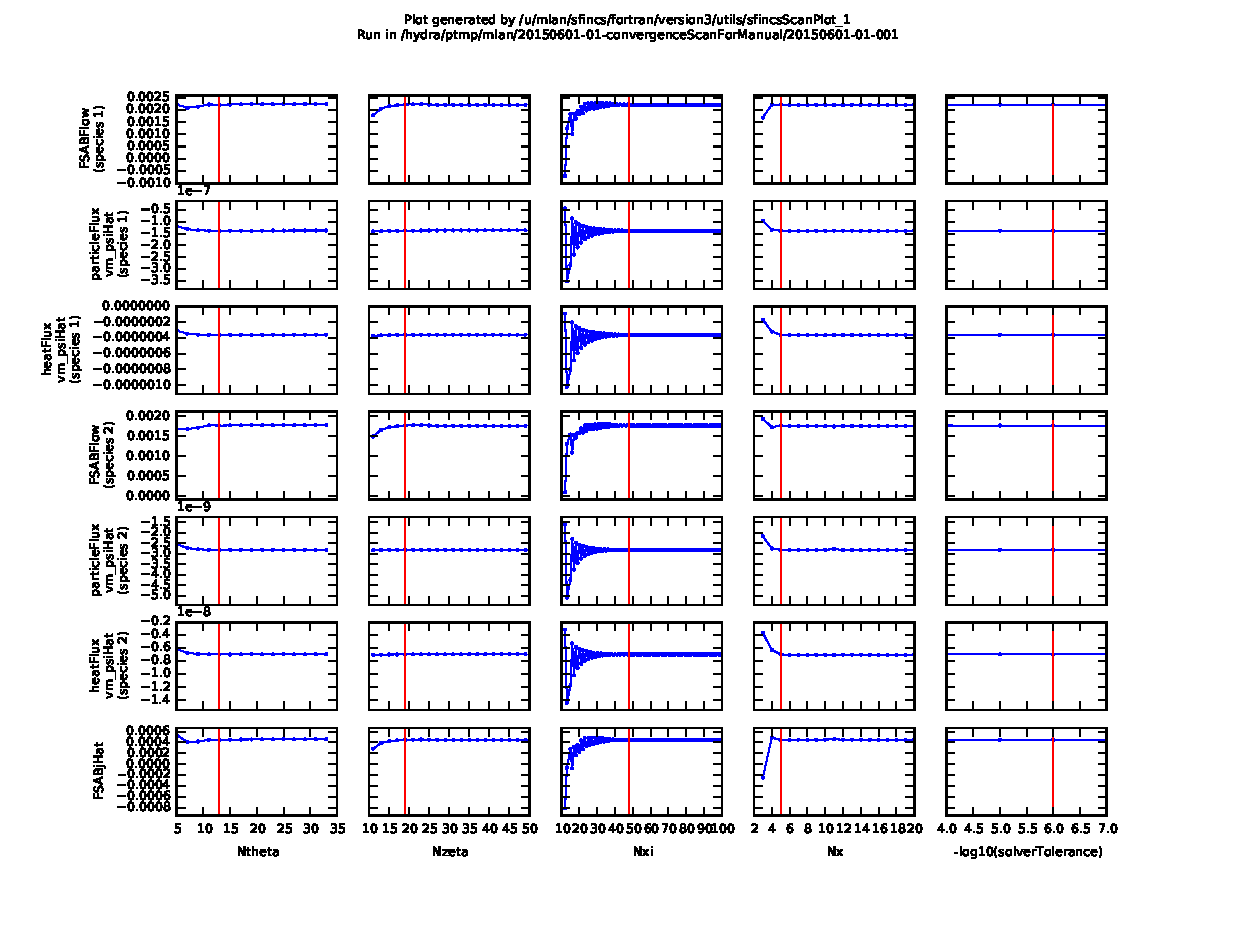
\includegraphics[width=1.0\textwidth]{sfincsConvergenceScan.pdf}
\mycaption{Plot generated by \sfincsScanPlot~showing a resolution convergence scan for the example
{\ttfamily geometryScheme4\_2species\_noEr}.
\label{fig:convergence}}
\end{center}
\end{figure}

To check how well the results of \sfincs~are converged with respect to the resolution
parameters, run \sfincsScan~with \parlink{scanType} = 1.
In this type of scan, a ``base case'' is first run at the
values of \Ntheta, \Nzeta, \Nxi, and \Nx~specified in the input file.
Then, each of these parameters will be varied in turn, holding the other parameters fixed.
The range of \Ntheta~in the scan is specified by the parameters \parlink{NthetaMinFactor},
\parlink{NthetaMaxFactor}, and \parlink{NthetaNumRuns}. 
Each of these three parameters is read by \sfincsScan~rather than by \sfincs~itself,
and so it must be prefaced by {\ttfamily !ss} in the input namelist file.
The ranges of \Nzeta, \Nxi, and \Nx~are set by parameters with analogous names,
as detailed in section \ref{sec:scanType1Parameters}.

For example, suppose you initially run \sfincsScan~with \Ntheta = 15, 
\parlink{NthetaMinFactor} = 0.7, \parlink{NthetaMaxFactor} = 1.5, and 
\parlink{NthetaNumRuns} = 5.
This will generate \sfincs~runs at \Ntheta = 11, 13, 15 (the base case), 19, and 23.
Notice that \sfincsScan~automatically ensures that only odd values are used.
(Only odd values of \Ntheta~and \Nzeta~are used internally in \sfincs.)
The maximum and minimum values for the scan, 11 and 23, are the nearest odd integers
to \Ntheta$\times$\parlink{NthetaMinFactor} and \Ntheta$\times$\parlink{NthetaMaxFactor} respectively.
Notice also that there are `gaps' at  \Ntheta = 17 and 21 since \sfincsScan~attempts to space the values
logarithmically rather than uniformly.

In addition to the 4 resolution parameters above, \sfincsScan~also allows the parameters
\parlink{solverTolerance}, \parlink{xMax}, and \parlink{NxPotentialsPerVth}
to be scanned.  The last two of these parameters are not used for the default \parlink{xGridScheme}
so it is usually unnecessary to scan them.  It is also usually unnecessary to scan \parlink{solverTolerance}
since the default value is usually robust.

A directory will be created for each run.  Each directory will contain
a copy of {\ttfamily input.namelist} in which \Ntheta, \Nzeta, \Nx, or \Nxi~has been
altered appropriately by \sfincsScan. Each directory will also contain a job file for the run.

You do not need to scan all variables. For example, if you do not wish to scan \Nx,
you can either set \parlink{NxNumRuns} = 0, or you can not specify
\parlink{NxNumRuns} in the {\ttfamily input.namelist} file.

Once the individual runs in the scan have begun to finish, you can plot the results by running \sfincsScanPlot.
You can plot the results before all the runs in the scan finish, although at least the base case
run must be completed.  Different quantities will be displayed depending on
\parlink{RHSMode} and \parlink{includePhi1}.

Typical convergence behavior is illustrated in figure \ref{fig:convergence},
showing the results of \sfincsScan~and \sfincsScanPlot~for the example
{\ttfamily geometryScheme4\_2species\_noEr}.
In this figure, a very large number of runs are included in the scan,
more than you would likely include in routine use of the code.
The red vertical lines emphasize the ``base case'' resolution parameters.
In each figure the spread is printed, defined as the maximum value $-$ minimum value,
divided by the value half-way between maximum and minimum.
If some runs have resolution below the base resolution,
the spread is also computed and printed
excluding runs below the base case resolution. (This is the second percentage printed in each plot,
and is usually more important than the first spread percentage.)
For all parameters scanned, the physical output quantities (particle flux, heat flux, etc)
do not visibly change on the scale of the plots when any of the resolution parameters
are increased beyond the base case value.  Indeed, the spread for each output quantity is $\le$ 3.5\%
when any resolution parameter is increased.
Thus, the results in the base case are well converged,
and so we can believe the results.
Observe in the figure that the output quantities tend to oscillate when \Nxi~is incremented by 1 and insufficient
\Nxi~is used. Results for even and odd \Nxi~converge to the same value, as one would hope.

\begin{figure}
\begin{center}
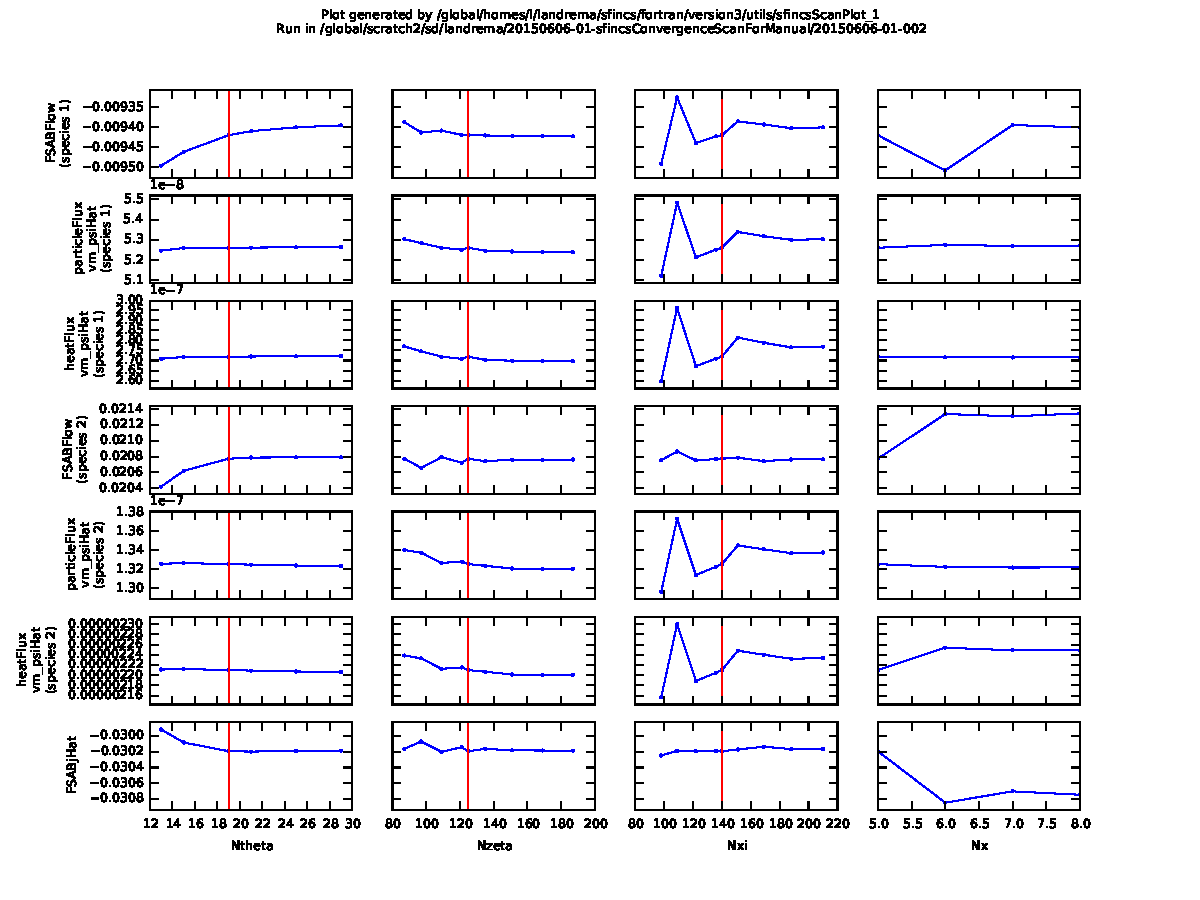
\includegraphics[width=1.0\textwidth]{sfincsConvergenceScan2.pdf}
\mycaption{Plot generated by \sfincsScanPlot~showing a typical resolution convergence scan for W7-X,
as you might generate during routine use of \sfincs.
\label{fig:convergence2}}
\end{center}
\end{figure}

For routine use of the code, it is not necessary to include as many
runs in the convergence scan as shown in figure \ref{fig:convergence},
and so a more typical routine scan would look like figure \ref{fig:convergence2}.
This scan is for a pure hydrogen plasma in the W7-X standard configuration, using \parlink{rN} = 0.19,
$n_e$ = $10^{20}$ m$^{-3}$, $T_i$ = 3.6 keV, and $T_e$ = 5.5 keV.
Notice the vertical scales in figure \ref{fig:convergence2} have suppressed zeros.
For all of the physical output quantities, the spread beyond the base case is $\le$ 3.4\%,
i.e. results change by no more than this percentage when each resolution
parameter is increased by 50\%. Hence we can conclude that 
the results are suitably converged at the base case resolution parameters.
The \sfincs~resolution parameters and \sfincsScan~parameters used for this scan were as follows:\\
{\ttfamily
\Ntheta = 19 \\
!ss \parlink{NthetaMinFactor} = 0.7 \\
!ss \parlink{NthetaMaxFactor} = 1.5 \\
!ss \parlink{NthetaNumRuns} = 6 \\
\Nzeta = 125 \\
!ss \parlink{NzetaMinFactor} = 0.7 \\
!ss \parlink{NzetaMaxFactor} = 1.5 \\
!ss \parlink{NzetaNumRuns} = 8 \\
\Nxi = 140 \\
!ss \parlink{NxiMinFactor} = 0.7 \\
!ss \parlink{NxiMaxFactor} = 1.5 \\
!ss \parlink{NxiNumRuns} = 8 \\
\Nx = 5 \\
!ss \parlink{NxMinFactor} = 1 \\
!ss \parlink{NxMaxFactor} = 1.6 \\
!ss \parlink{NxNumRuns} = 4 \\
}
These \sfincsScan~parameters are good for routine convergence tests, although the \sfincs~parameters proper
(\Ntheta, \Nzeta, \Nxi, and \Nx) should be tailored to your application.

If you wish to add more runs to the scan at a later time,
you can alter the relevant \sfincsScan~parameters in the original {\ttfamily input.namelist}~file
and run \sfincsScan~again from the original directory.  The \sfincsScan~code will automatically detect which runs
have already been submitted, so duplicate runs will not be generated.
For example, consider the scan of \Ntheta~described at the start of this section,
and suppose you wish to fill in the gaps at \Ntheta = 17 and 21 in the original scan.
To do this, you could set \parlink{NthetaNumRuns} to a large number like 100
and re-run \sfincsScan.  Since \sfincsScan~intelligently avoids duplication,
the only new runs generated will be  \Ntheta = 17 and 21.

If you are ultimately intending to scan $E_r$, you probably only need to run a convergence scan
at a single value of $E_r$.  This is because the resolution requirements of \sfincs~are not sensitive to
$E_r$, as discussed above.
Also, if you are ultimately intending to run \sfincs~at a range of minor radii,
it is reasonably to only run a convergence scan at a single radius close to the magnetic axis.
This is because the typically peaked shape of the temperature profile means that
collisionality is lowest near the axis.  Since the resolution requirements of \sfincs~are most
demanding at low collisionality, then if the code is converged at the radius of lowest collisionality,
it should be converged at all radii.

\section{Examples of resolution requirements}

To estimate the appropriate resolution parameters for various circumstances, you can look at
the examples in the \path{sfincs/fortran/version3/examples/} directory. 
Some other examples of appropriate resolution parameters are given in the following sections.

\subsection{W7-X with anticipated experimental density and temperature}
\label{sec:w7xresolution}

The following parameters have been extensively tested with W7-X geometry for densities near $10^{20}$ m$^{-3}$
and temperatures up to 6 keV, and found to give convergence to $\sim 3$\% (as shown in figure \ref{fig:convergence2}):\\
{\ttfamily
\Ntheta = 19 \\
\Nzeta = 125 \\
\Nxi = 140 \\
\Nx = 5 \\
}
Note that at lower temperature and/or higher density, the collisionality will be higher,
so comparable convergence could be achieved at lower \parlink{Nzeta} and \parlink{Nxi}.
Conversely, at higher temperatures and/or lower desntiy, the collisionality will be lower,
so comparable convergence would likely require higher  \parlink{Nzeta} and \parlink{Nxi}.

\subsection{Figure 3 of the original SFINCS paper}

For figure 3 in Ref \cite{sfincsPaper}, corresponding to a pure plasma in W7-X with $n = 6.6\times 10^{19}$ m$^3$ and $T_i = T_e = 1$ keV,
the calculations used\\
{\ttfamily
\Ntheta = 19 \\
\Nzeta = 59 \\
\Nxi = 60 \\
\Nx = 5. \\
}
Note the lower values of  \parlink{Nzeta} and \parlink{Nxi} used compared to section \ref{sec:w7xresolution},
which were sufficient since the temperatures were lower.

\subsection{Figure 4 of the original SFINCS paper}

For figure 4 in Ref \cite{sfincsPaper}, corresponding to a collisionality scan in LHD,
the following resolution parameters were used:

\centerline{
\begin{tabular}{c|c|c|c|c}
\parlink{nuPrime} & \Ntheta & \Nzeta & \Nxi & \Nx \\
\hline
0.001 & 85 & 41 & 103 & 5 \\
0.01 & 21 & 25 & 70 & 5 \\
0.1 & 15 & 13 & 37 & 5 \\
0.3 & 15 & 13 & 34 & 6 \\
1 & 13 & 13 & 13 & 8 \\
10 & 15 & 13 & 13 & 8 \\
100 & 15 & 13 & 13 & 8
\end{tabular}
}

\subsection{Figure 5 of the original SFINCS paper}

For figure 5 in Ref \cite{sfincsPaper}, corresponding to a collisionality scan in W7-X,
the following resolution parameters were used:

\centerline{
\begin{tabular}{c|c|c|c|c}
\parlink{nuPrime} & \Ntheta & \Nzeta & \Nxi & \Nx \\
\hline
0.001 & 29 & 83 & 180 & 5 \\
0.01  & 11 & 64 & 100 & 5 \\
0.1   & 11 & 37 & 37  & 5 \\
0.3   & 11 & 29 & 30  & 5 \\
1     & 13 & 31 & 24  & 6 \\
10    & 13 & 35 & 12  & 7 \\
100   & 11 & 37 & 13  & 8
\end{tabular}
}
 

\renewcommand{\chaptermark}[1]{\markboth{\sc{Appendix\ \thechapter.\ #1}}{}}
\appendix
\setcounter{tocdepth}{0}

% Appendices can go here:
%\chapter{Details for specific computing systems}

\section{NERSC edison}

\section{IPP hydra}

\section{Chalmers University - Glenn cluster}

 
\lhead[\thepage]{\sc Bibliography}
\rhead[\sc Bibliography]{\thepage}
\bibliography{SFINCSUserManual}
\bibliographystyle{mymanual}
\end{document}

